% !TEX encoding = UTF-8 Unicode
%!TEX program = xelatex

% Name           : hsrm-beamer-demo.sty
% Author         : Benjamin Weiss (benjamin.weiss@kreatiefton.de)
% Version        : 0.4
% Created on     : 05.05.2013
% Last Edited on : 24.03.2014
% Copyright      : Copyright (c) 2013-2014 by Benjamin Weiss. All rights reserved.
% License        : This file may be distributed and/or modified under the
%                  GNU Public License.
% Description    : HSRM beamer theme demonstration. Also includes a short 
%                  Tutorial regarding the beamer class.
\documentclass[xcolor=table]{beamer}
%\documentclass[compress]{beamer}
%--------------------------------------------------------------------------
% Common packages
%--------------------------------------------------------------------------
%\usepackage[spanish]{babel}
\usepackage[spanish, mexico,es-lcroman]{babel}
\usepackage[utf8]{inputenc}

\usepackage{graphicx}
\usepackage{multicol}
\usepackage{multirow}
% Erweiterte Tabellenfunktionen
\usepackage{tabularx,ragged2e}
\usepackage{booktabs}

%\usepackage[table,xcdraw]{xcolor}
% Listingserweiterung
\usepackage{listings}
\usepackage{animate}
\lstset{ %
language=[LaTeX]TeX,
basicstyle=\normalsize\ttfamily,
keywordstyle=,
numbers=left,
numberstyle=\tiny\ttfamily,
stepnumber=1,
showspaces=false,
showstringspaces=false,
showtabs=false,
breaklines=true,
frame=tb,
framerule=0.5pt,
tabsize=4,
framexleftmargin=0.5em,
framexrightmargin=0.5em,
xleftmargin=0.5em,
xrightmargin=0.5em
}

%--------------------------------------------------------------------------
% Load theme
%--------------------------------------------------------------------------
\usetheme{hsrm}
\usepackage{dtklogos} % must be loaded after theme
\usepackage{tikz}
\usetikzlibrary{mindmap,backgrounds}

%--------------------------------------------------------------------------
% General presentation settings
%--------------------------------------------------------------------------
\title{Defensa de tesis}
\subtitle{Desarrollo de un c\'{o}dec \\para la transmisi\'{o}n de audio cardiaco\\ sobre redes de bajas tasas de datos}
\date{\today}
\author{Roilhi Frajo Ibarra Hern\'{a}ndez}
\institute{Departamento de Electr\'{o}nica y Telecomunicaciones\\Divisi\'{o}n de F\'{i}sica Aplicada}

%--------------------------------------------------------------------------
% Notes settings
%--------------------------------------------------------------------------
\setbeameroption{show notes}

\begin{document}
%--------------------------------------------------------------------------
% Titlepage
%--------------------------------------------------------------------------

%\maketitle
\beamertemplatenavigationsymbolsempty
\begin{frame}[plain]
	\titlepage
\end{frame}
\begin{frame}{Comit\'e evaluador de tesis}
\begin{itemize}
	\item Dr. Miguel \'Angel Alonso Ar\'evalo
		\begin{itemize}
			\item \emph{Director de tesis}
		\end{itemize}
	\item Dr. Salvador Villarreal Reyes
		\begin{itemize}
			\item \emph{Miembro del comit\'e}
		\end{itemize}	
	\item Dr. Roberto Conte Galv\'an
		\begin{itemize}
			\item \emph{Miembro del comit\'e}
		\end{itemize}
	\item Dr. Jon\'as D. de Basabe Delgado
		\begin{itemize}
			\item \emph{Miembro externo del comit\'e}
		\end{itemize}
\end{itemize}
\end{frame}

%--------------------------------------------------------------------------
% Table of contents
%--------------------------------------------------------------------------

\begin{frame}{Contenido}
	\tableofcontents[hideallsubsections]
\end{frame}
%==============================================================================
%-----------------------------------------------------------------------
%	   _
%	  | |                         |                   o
%	  | | _  _  _|_  ,_    __   __|          __   __      _/   _  _
%	_ |/ / |/ |  |  /  |  /  \_/  |  |   |  /    /    |  /  \_/ |/ |
%	\_/\/  |  |_/|_/   |_/\__/ \_/|_/ \_/|_/\___/\___/|_/\__/   |  |_/
%-----------------------------------------------------------------------

\section{Introducci\'on}

% ----------------------------------------------------------------------
\begin{frame}{Introducci\'on}
	\begin{itemize}
	\item<2-> \emph{Enfermedades cardiovasculares (CVD's)}  $\Rightarrow$ son las principales causa de muerte en el mundo seg\'un la OMS\footnote{Datos actualizados hasta marzo del 2013.}.
	
	\item<3-> En 2008 fallecieron 17.3 millones de personas en el mundo a causa de alguna CVD.
	\end{itemize}\pause
		\begin{figure}
		\centering
		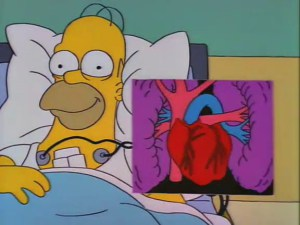
\includegraphics[width=0.5\textwidth]{homers_heart.jpg}
	\end{figure}
\end{frame}

\begin{frame}{Fonocardiograma}
	\begin{exampleblock}{Auscultaci\'on}
		M\'etodo econ\'omico, accesible y confiable en la detecci\'on de cardiopat\'ias. Se obtiene en \'este una se\~nal de audio llamada \emph{fonocardiograma (PCG)} que indica la actividad de las v\'alvulas cardiacas.	
	\end{exampleblock}
			\begin{figure}
		\centering
		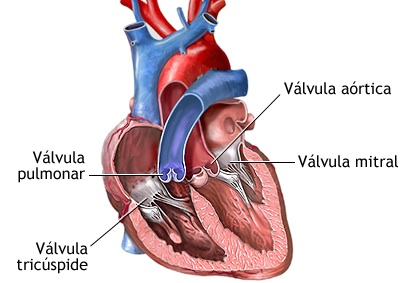
\includegraphics[width=0.55\textwidth]{valvulas_cardiacas.jpg}
	\end{figure}
\end{frame}


\begin{frame}{Fonocardiograma}
	Ciclo cardiaco $\Rightarrow$ Se consideran dos sonidos o eventos principales.
		\begin{table}
			\begin{tabular}{c|c|c}
			\hline
			Evento & Duraci\'on (s)& Frecuencias (Hz) \\
			\hline
			s1     & 0.1-0.12      & 20-150\\
			\hline
			s2     & 0.08-0.14	   & 50-60 \\
			\hline
			\end{tabular}
		\end{table}
	\textbf{Se\~nal cuasi-estacionaria}: Los ciclos son altamente consistentes y muy similares en duraci\'on, tiempo y forma.
\end{frame}

\begin{frame}{Fonocardiograma}
	Patolog\'ia cardiaca $\Rightarrow$ Da\~no en las v\'alvulas, cambio en el flujo sangu\'ineo y en la frecuencia del sonido.
		\begin{figure}
			\centering
		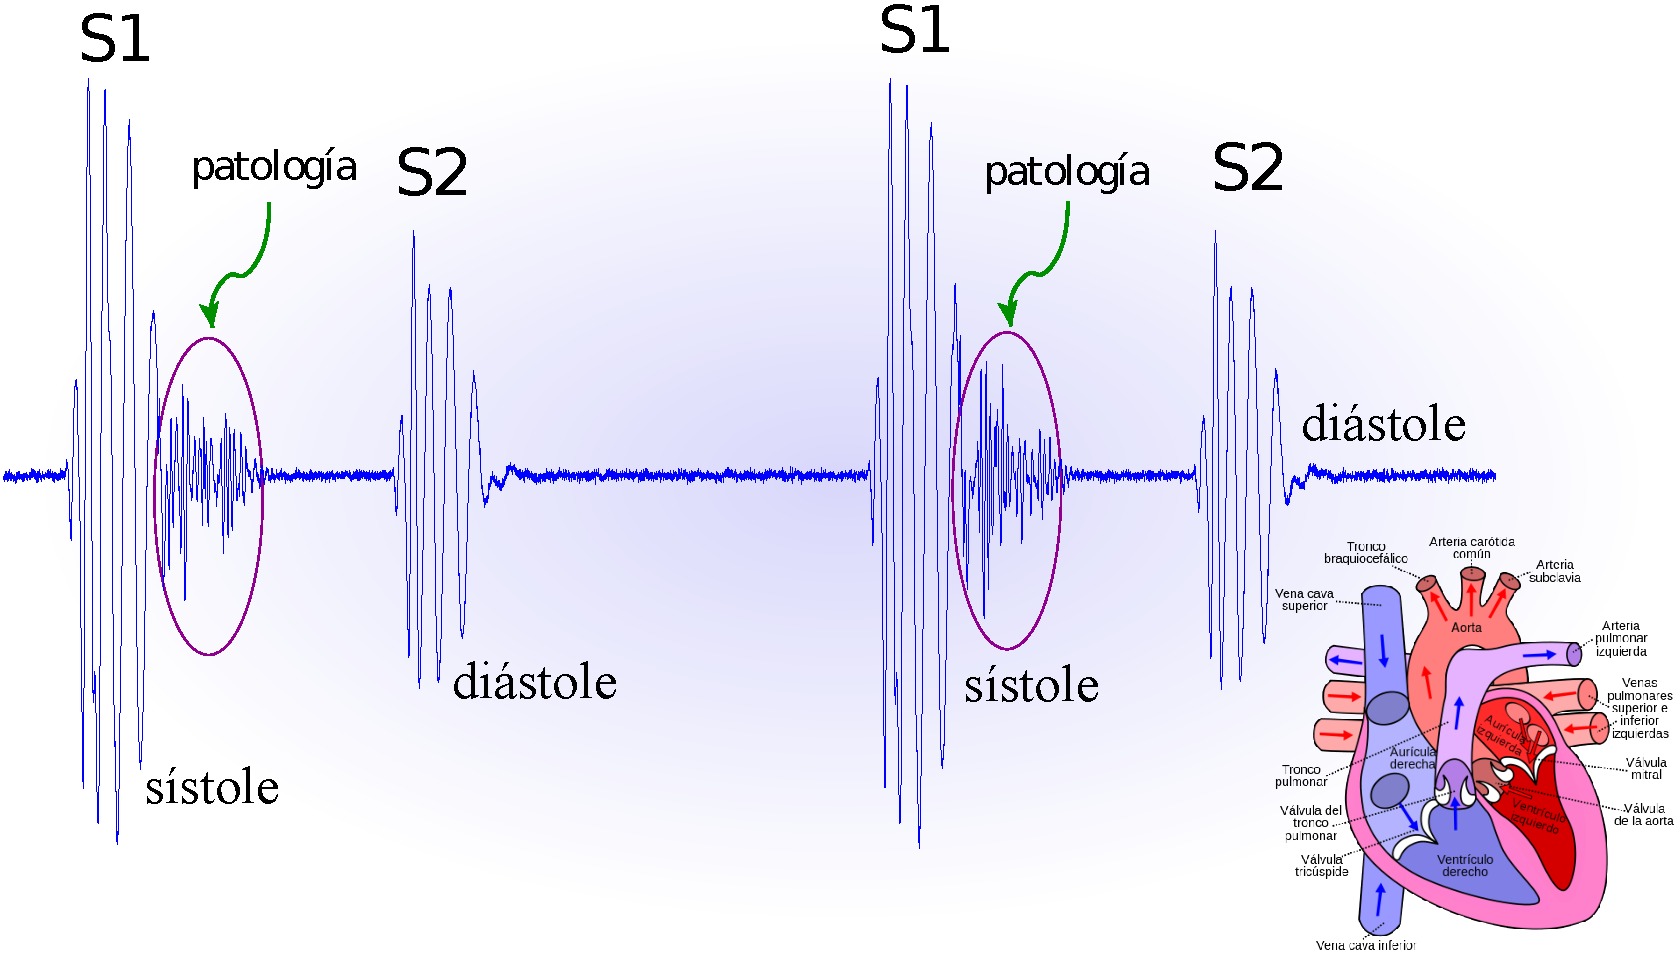
\includegraphics[scale=0.37]{pcg_waveform.pdf}
		\end{figure}
\end{frame}

\begin{frame}{Fonocardiograma}
	La mayor parte de la energ\'ia del PCG no es audible, se encuentra por debajo del umbral de audici\'on.
	
	\begin{figure}
	\centering
	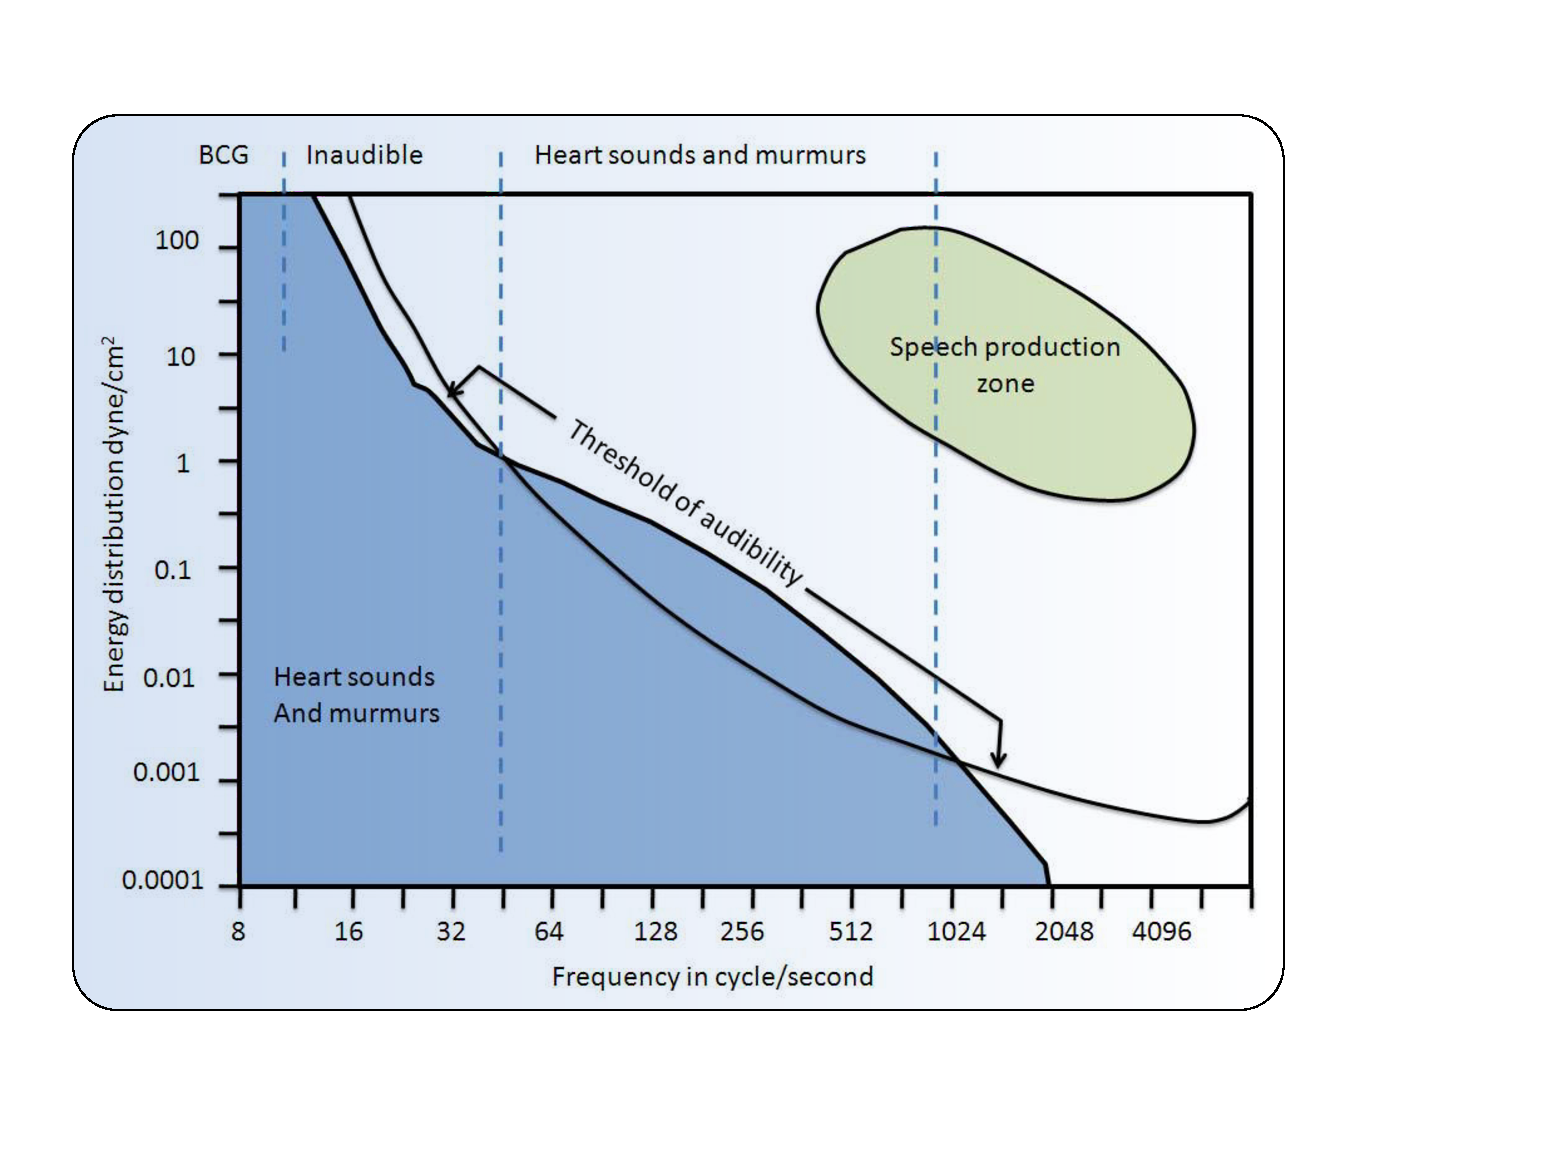
\includegraphics[width=0.85\textwidth]{PCG_audition.pdf}
	\end{figure}
\end{frame}

\begin{frame}{Fonocardiograma}
	\begin{itemize}
		\item<2-> La digitalizaci\'on del PCG permite analizarle en el plano tiempo-frecuencia con m\'as precisi\'on.
		\item<3-> El contenido frecuencial del fonocardiograma no rebasa los 2,000 Hz a\'un con patolog\'ias.
	\end{itemize}\pause
	\begin{figure}
		\centering
		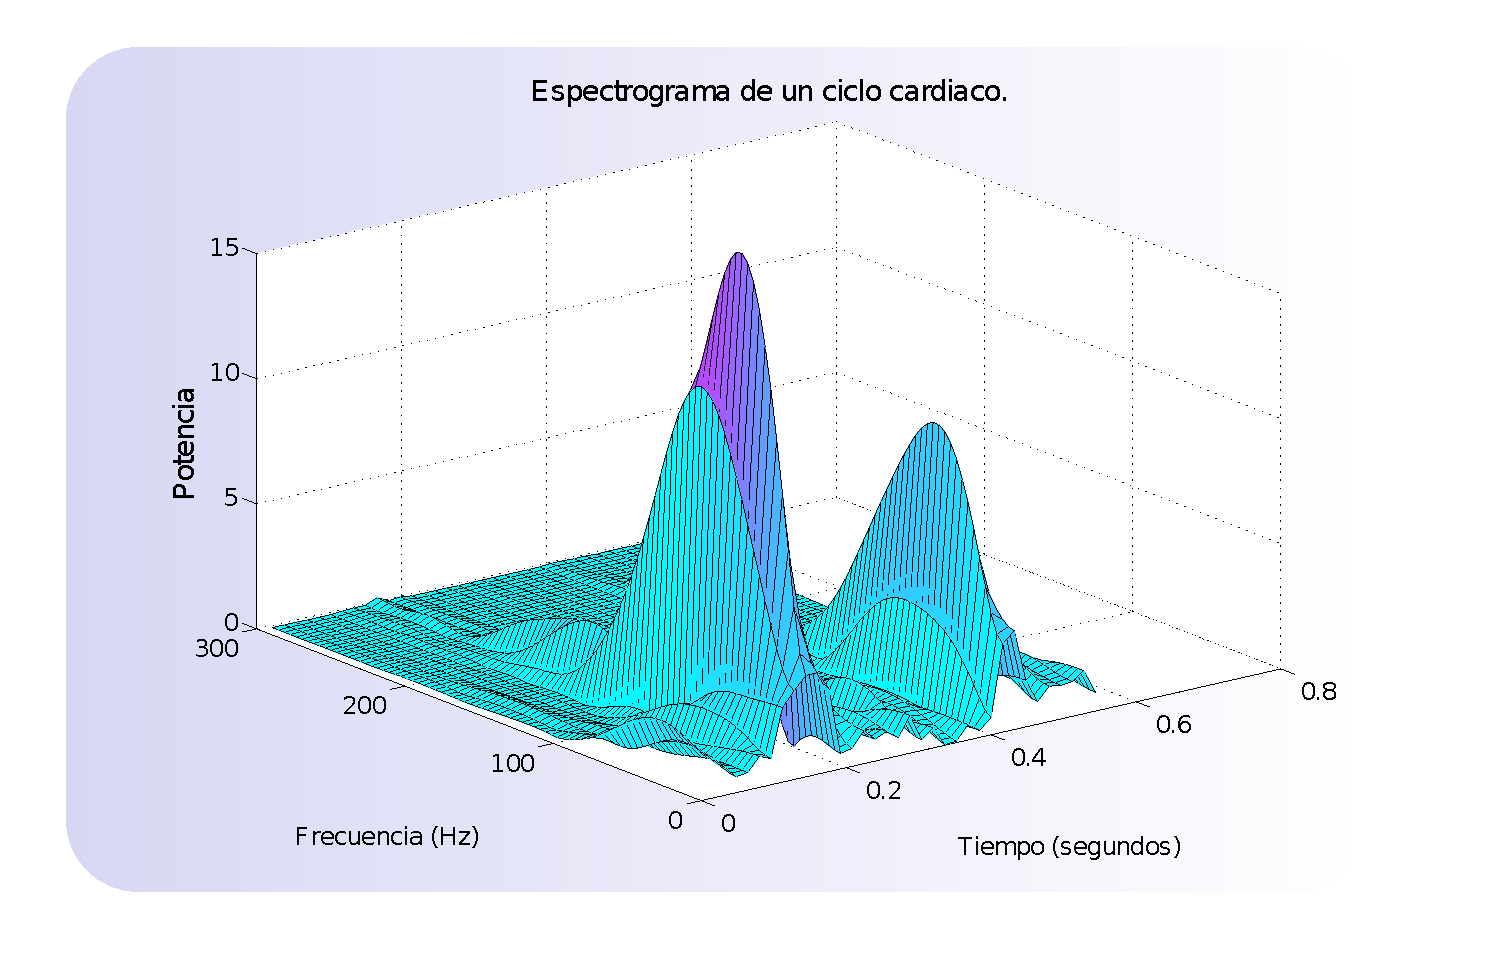
\includegraphics[width=0.8\textwidth]{spectrogram_PCG.pdf}
	\end{figure}
\end{frame}

\begin{frame}{Planteamiento del problema}
	\begin{itemize}
		\item<2-> Los codificadores existentes est\'an dise\~nados para audio en general. 
		\item<3-> Los recursos son excesivos para representar al PCG en frecuencia. 
	\end{itemize}\pause
	\begin{exampleblock}{Objetivo de la tesis}
		Dise\~nar\ un c\'odec (codificador-decodificador) tipo param\'etrico adaptado al audio cardiaco para su transmisi\'on sobre redes de bajas tasas de datos. 			
	\end{exampleblock}
\end{frame}

\begin{frame}
	\begin{itemize}
		\item<2-> Anteriormente se han modelado con \'exito se\~nales PCG de manera determin\'istica mediante Matching Pursuit.
		\item<3-> Se crey\'o que el modelo determinista era suficiente para representar la informaci\'on contenida en la se\~nal.
		\item<4-> Se propone en este trabajo el modelado de la suma de dos partes:
					$$
						 PCG= Parte_{determinista} + Parte_{estocastica}$$									
					
		\item<5-> No se ha encontrado alg\'un codificador para audio cardiaco con dichas caracter\'isticas.
	\end{itemize}
\end{frame}

\begin{frame}{Estructura del c\'odec}
Etapa de codificaci\'on
	\begin{figure}
		\centering
		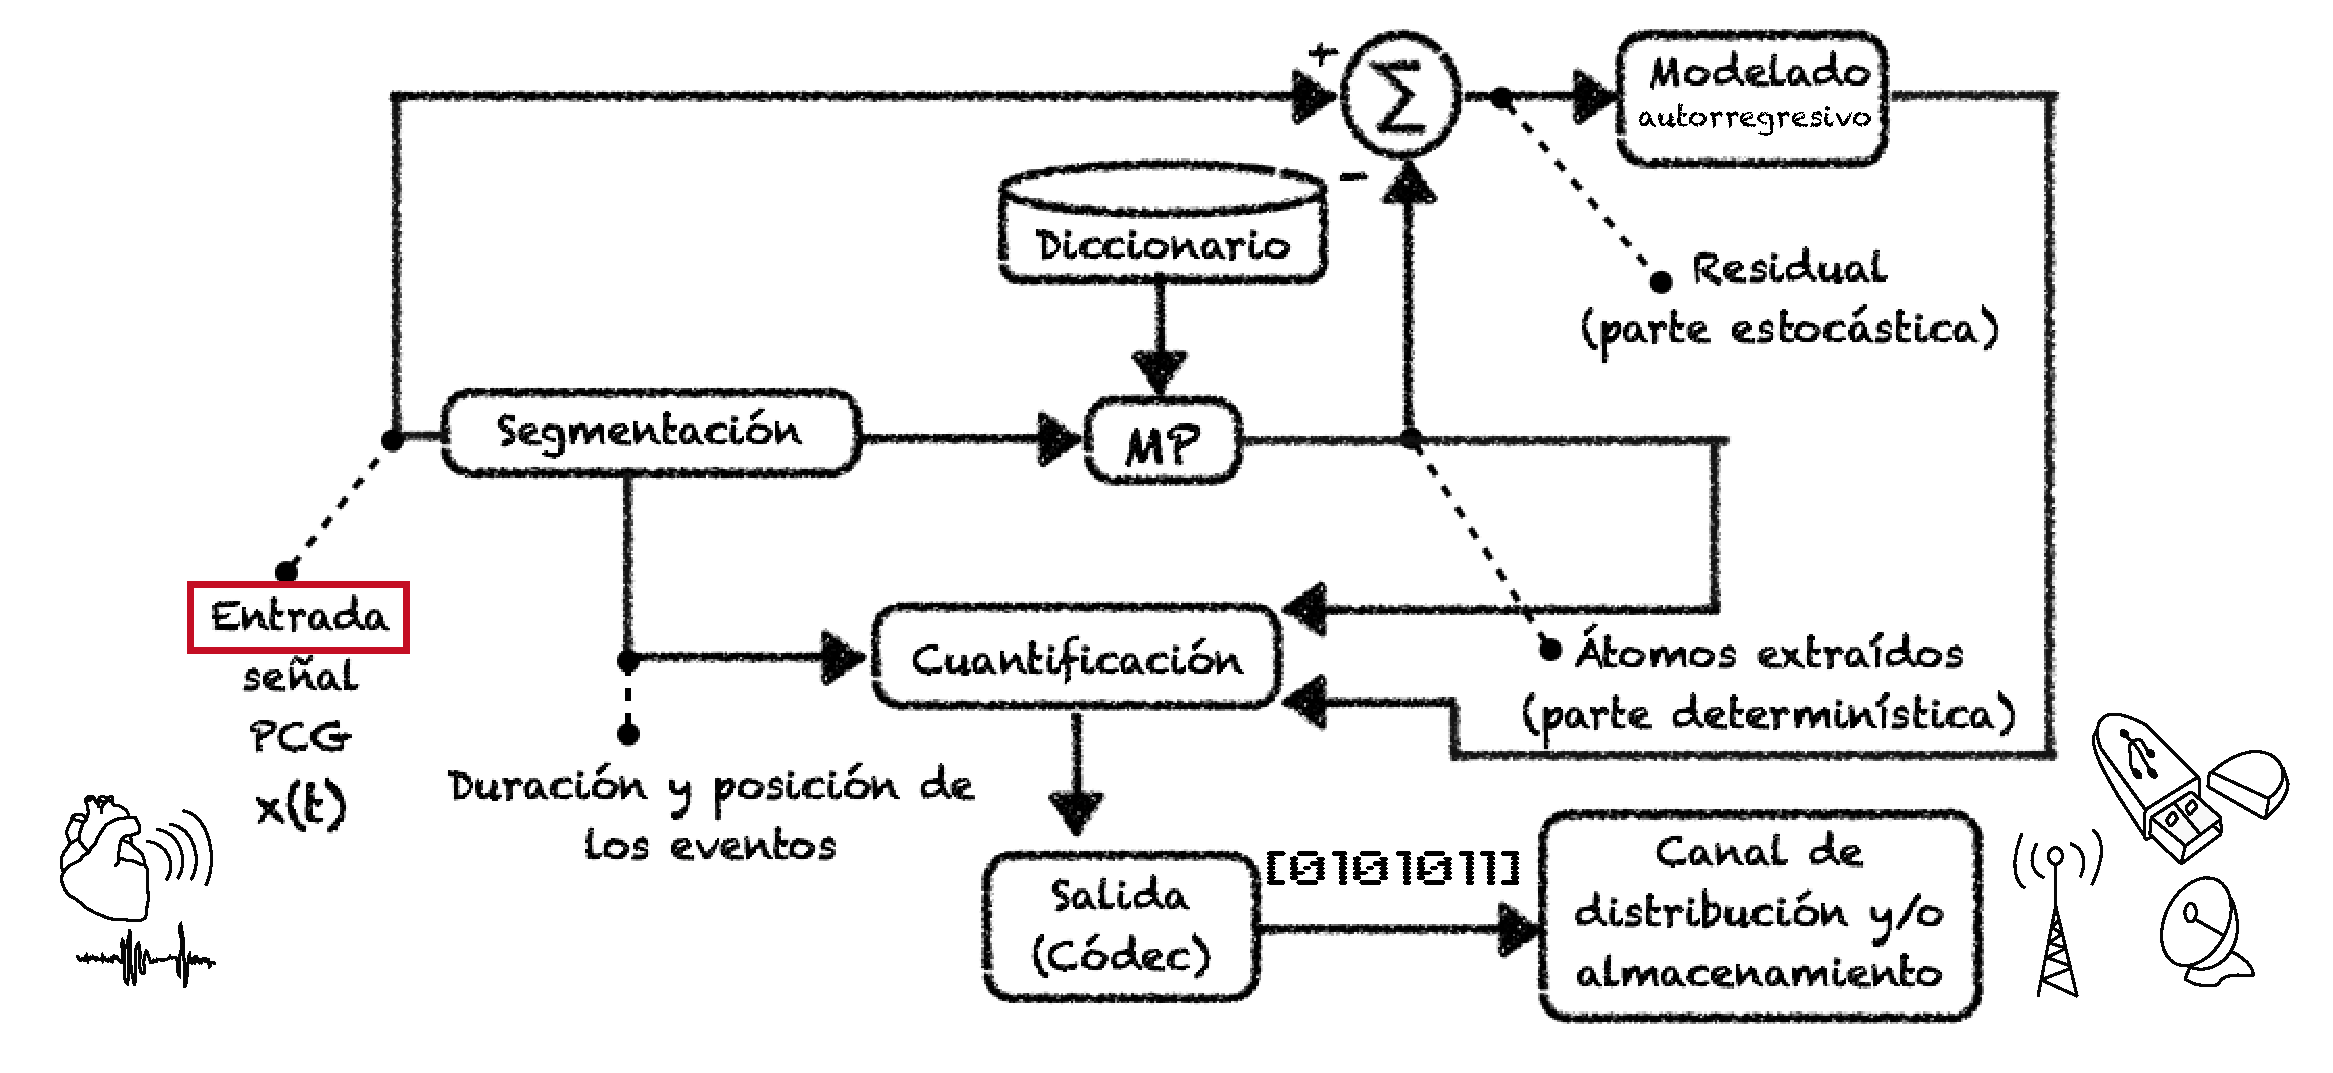
\includegraphics[scale=0.28]{codificador2.pdf}
	\end{figure}
\end{frame}

\begin{frame}{Estructura del c\'odec}
Etapa de decodificaci\'on
	\begin{figure}
		\centering
		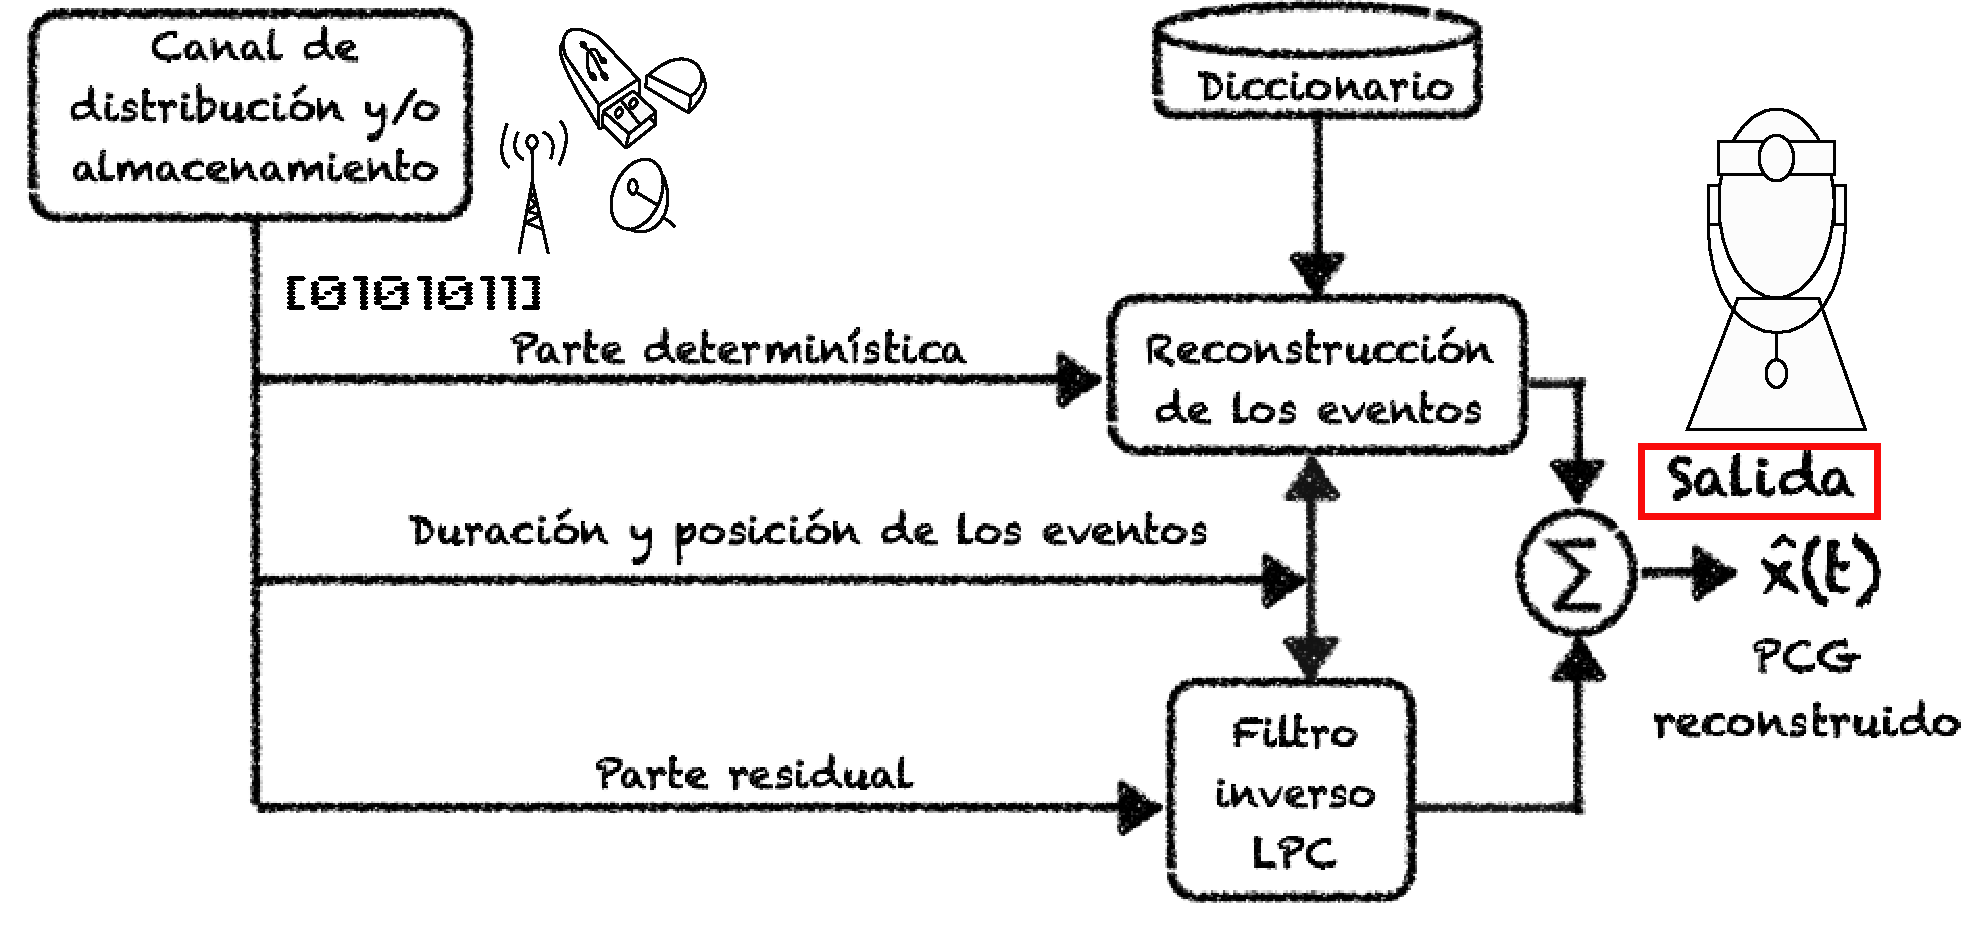
\includegraphics[scale=0.34]{decodificador2.pdf}
	\end{figure}
\end{frame}
% -----------------------------------------------------------------------------
%------------------------------------------------------------------------------
%	 ,__ __                   _
%	/|  |  |          |      | |          |
%	 |  |  |   __   __|   _  | |  __,   __|   __       _   __,   ,_  _|_  _
%	 |  |  |  /  \_/  |  |/  |/  /  |  /  |  /  \_   |/ \_/  |  /  |  |  |/
%	 |  |  |_/\__/ \_/|_/|__/|__/\_/|_/\_/|_/\__/    |__/ \_/|_/   |_/|_/|__/
%	                                                /|
%	                                                \|
%	
%	   |                              o          /         o
%	 __|   _ _|_  _   ,_    _  _  _       _  _       , _|_     __   __,
%	/  |  |/  |  |/  /  |  / |/ |/ |  |  / |/ |  |  / \_|  |  /    /  |
%	\_/|_/|__/|_/|__/   |_/  |  |  |_/|_/  |  |_/|_/ \/ |_/|_/\___/\_/|_/
%-------------------------------------------------------------------------------
%-------------------------------------------------------------------------------
\section{Modelado de la parte determin\'istica}
% ----------------------------------------------------------------------
\begin{frame}{Representaci\'on dispersa de se\~nales}

\alert{Idea principal:} Extraer informaci\'on compacta a partir de conjuntos masivos de datos.
		\begin{exampleblock}{Representaci\'on dispersa}
			La mayor\'ia o totalidad de la informaci\'on es representada por una
			combinaci\'on lineal de formas de onda llamadas \'atomos.
			$$x(t)=\sum_{k}u_{k}\mathbf{\phi}_{k}(t)$$
			o en forma matricial:
			$$\vec{x}=\Phi \vec{u},$$
			donde $x$ es la se\~nal a representar, $\phi$ el $k$-\'esimo \'atomo y $\Phi$ el conjunto \'atomos o 							\emph{diccionario}; $\vec{u}$ es un vector significativo para realizar la representaci\'on.
		\end{exampleblock}
\end{frame}
	

\begin{frame}{Representaci\'on dispersa de se\~nales}
	\begin{itemize}
		\item<2-> Base sobrecompleta $\Rightarrow$ existe una cantidad infinita de $\vec{u}$ que generan la misma $\vec{x}$.
		\item<3-> Mayor inter\'es en los $\vec{u}$ dispersos, estos son los que contienen el menor n\'umero $K$, de elementos 					  distintos de cero.
		\end{itemize}\pause
    \begin{figure}[h!]
    \centering
      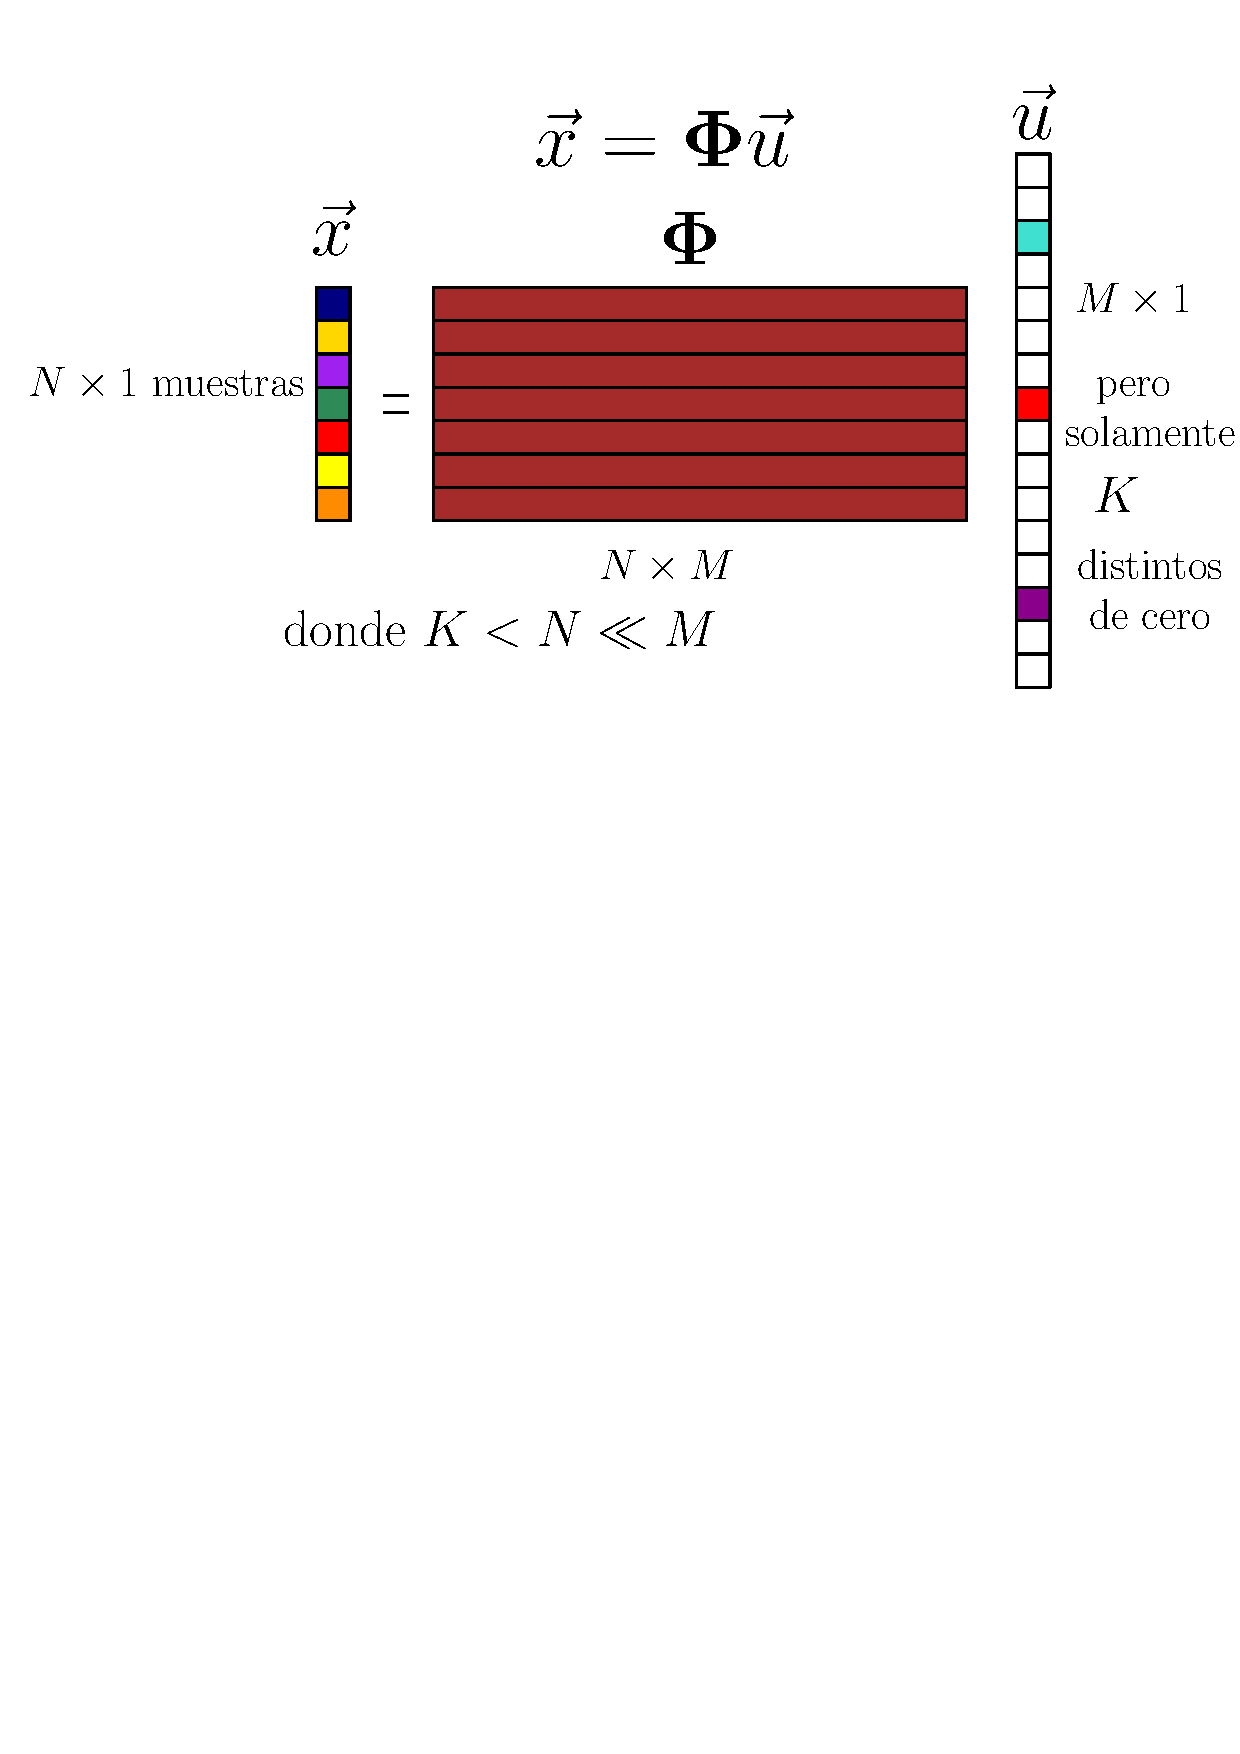
\includegraphics[scale=0.45]{sparse_diagram.pdf}
    \end{figure}
\end{frame}

\begin{frame}{Matching Pursuit}
	\begin{itemize}
		\item<2-> Algoritmo de RD seleccionado en este trabajo. 
		\item<3-> \emph{Descompone} o representa una se\~nal $x(t)$ en una combinaci\'on lineal de \'atomos y un t\'ermino residual:
					\begin{figure}
						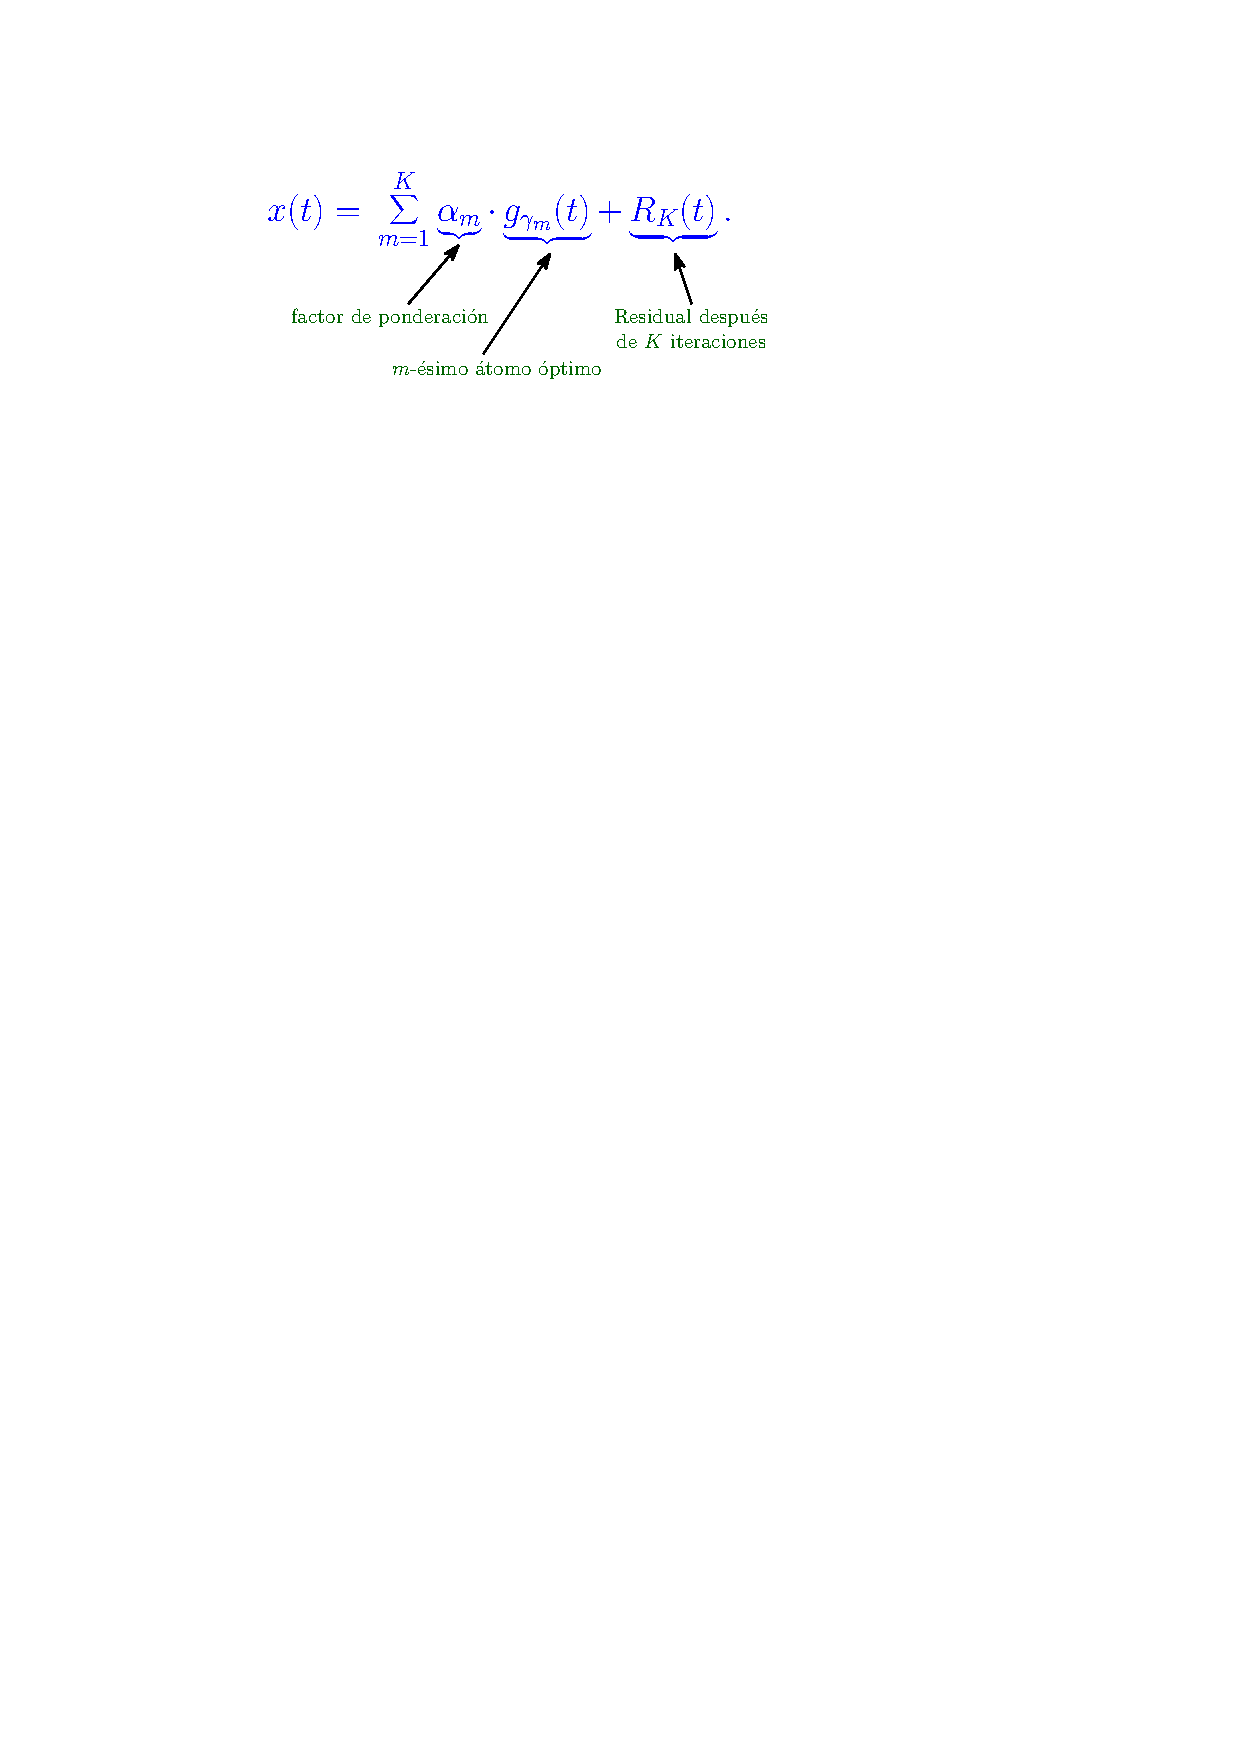
\includegraphics[scale=0.95]{MP_equation.pdf}
					\end{figure}
		\item<4-> Selecciona en cada iteraci\'on los \'atomos que mejor coincidan (\emph{best-match}) con la estructura de la se\~nal.
		\item<5-> Una vez seleccionado el \'atomo que mejor coincida se extrae (resta) de $x(t)$ y comienza de nuevo el proceso hasta cumplir un criterio para detener el algoritmo. 
		
	\end{itemize}
\end{frame}

\begin{frame}{Matching Pursuit}
	\begin{itemize}
		\item<2-> Es importante la selecci\'on de un diccionario adecuado para las descomposiciones en MP.
		\item<3-> Se ha encontrado que los diccionarios de Gabor presentan elementos con caracter\'isticas similares a las 			  de la se\~nal a modelar.
		\item<4-> Los \emph{\'atomos} de Gabor son ondas cosenoidales bien concentradas en tiempo y frecuencia obtenidas 			  por:
				\begin{itemize}
					\item<5-> Dilataci\'on 
					\item<6-> Modulaci\'on
					\item<7-> Traslaci\'on
				\end{itemize}
				de un impulso gaussiano.
	\end{itemize}
\end{frame}

\begin{frame}{\'Atomos de Gabor}
				Forma de onda de un \'atomo de Gabor:
				$$ g_\gamma(t)=\frac{1}{\sqrt{s}}w\left(\frac{t-u}{s}\right)e^{j2\pi\xi(t-u)},$$
				donde: $w=\sqrt[4]{2}e^{-\pi t^2}$ y adem\'as $\int_{-\infty}^{\infty}{|w(t)|^2}dt=1$
	\begin{figure}
	\centering
	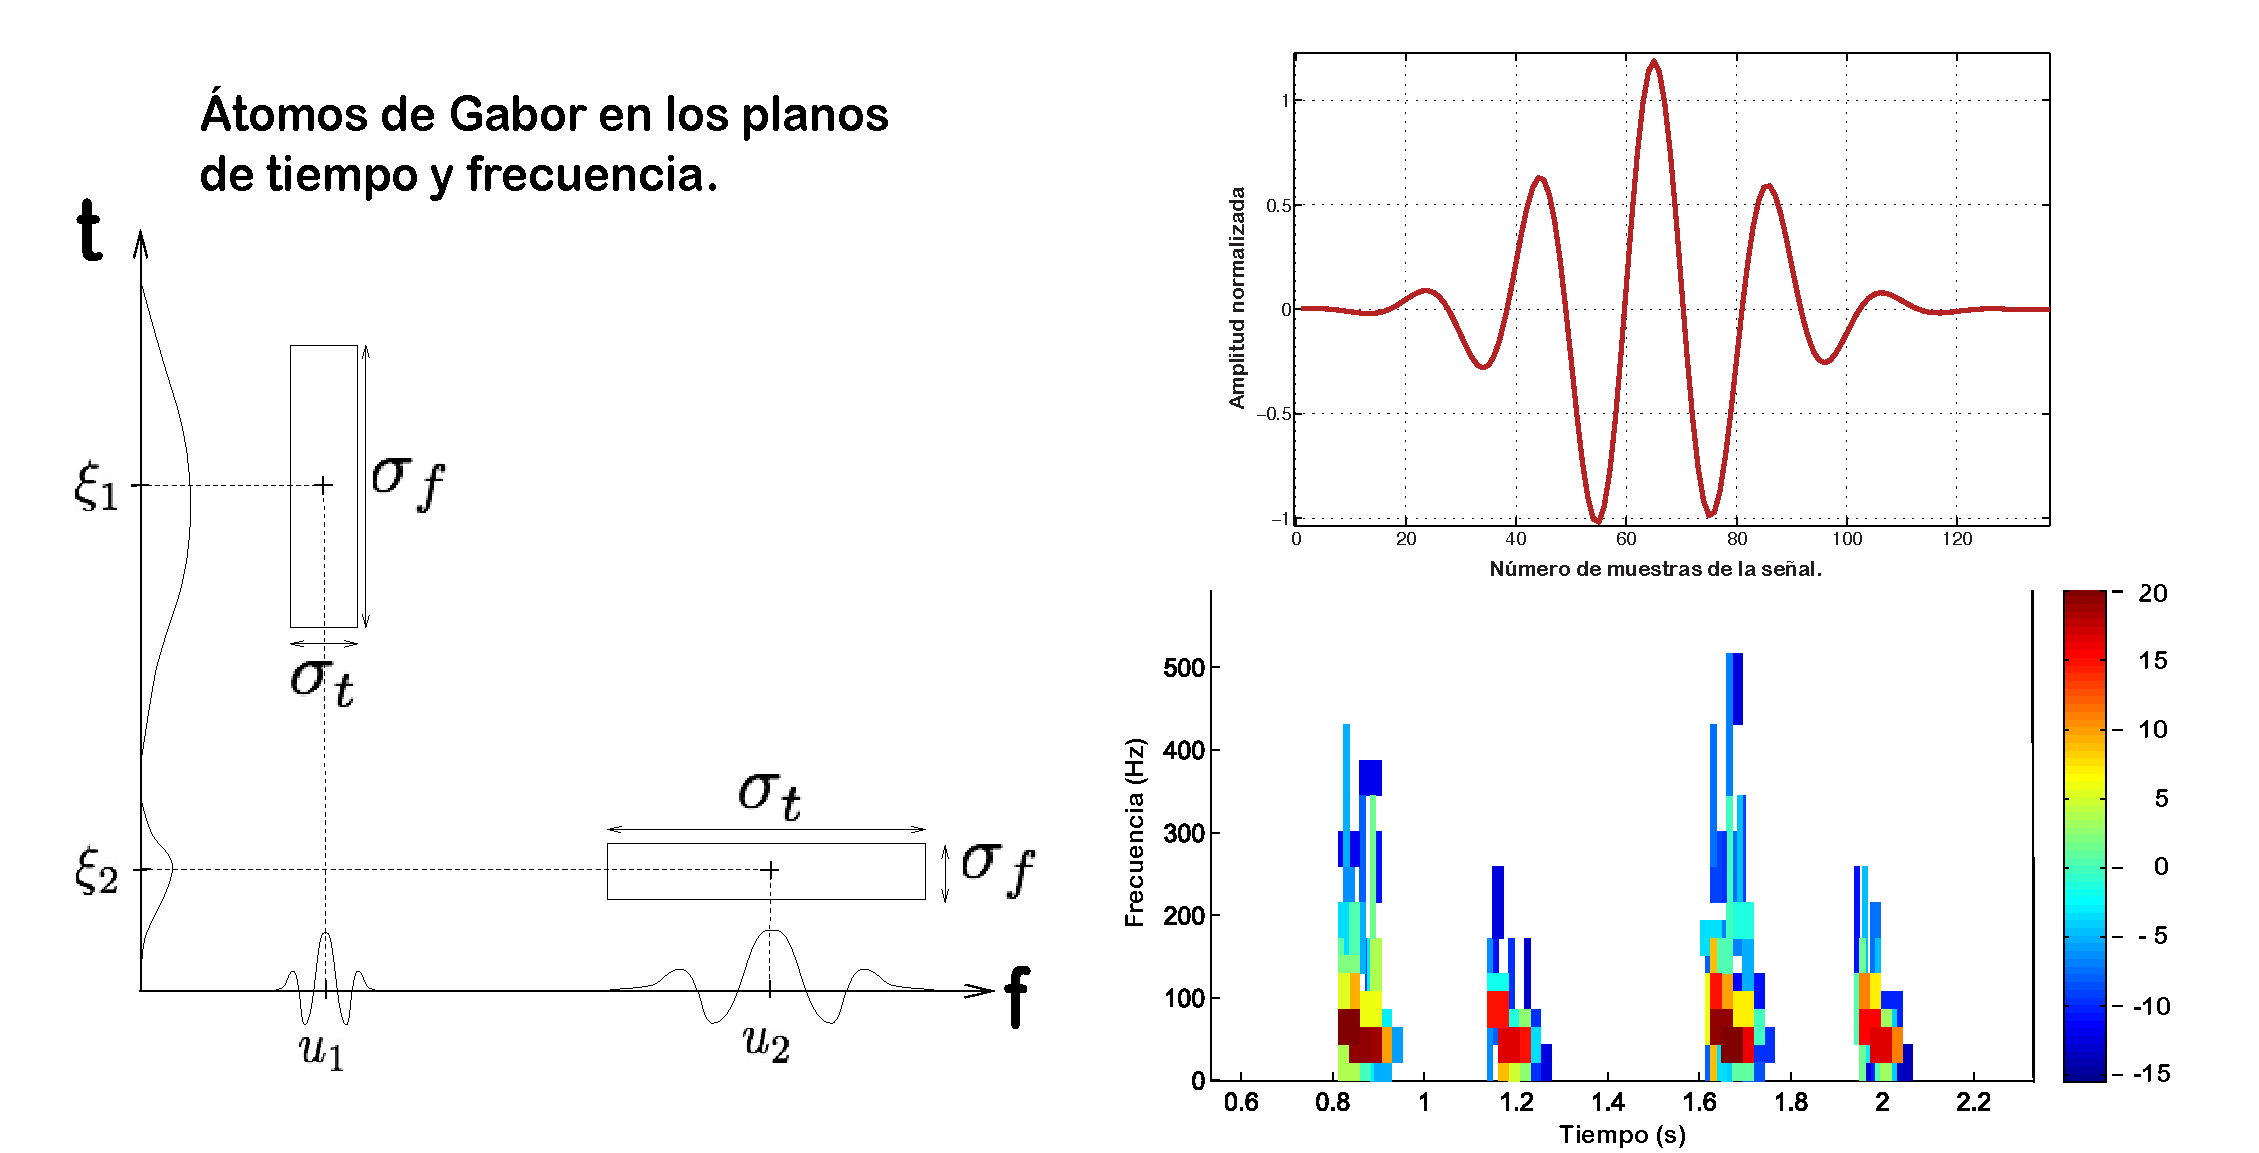
\includegraphics[width=0.98\textwidth]{gaborAtoms.pdf}
	\end{figure}
\end{frame}

\begin{frame}{Descomposici\'on MP de un evento cardiaco}
\begin{center}
	\animategraphics[controls,autoplay,loop,height=7cm]{1}{matlab/MPpcg}{1}{31} 
\end{center}
\end{frame}

\begin{frame}{Descomposici\'on MP de un evento cardiaco.}
Se ha desarrollado la reconstrucci\'on de la forma de onda de eventos cardiacos 
con precisi\'on mediante Matching Pursuit y \'atomos de Gabor. 
	\begin{figure}
	\centering
	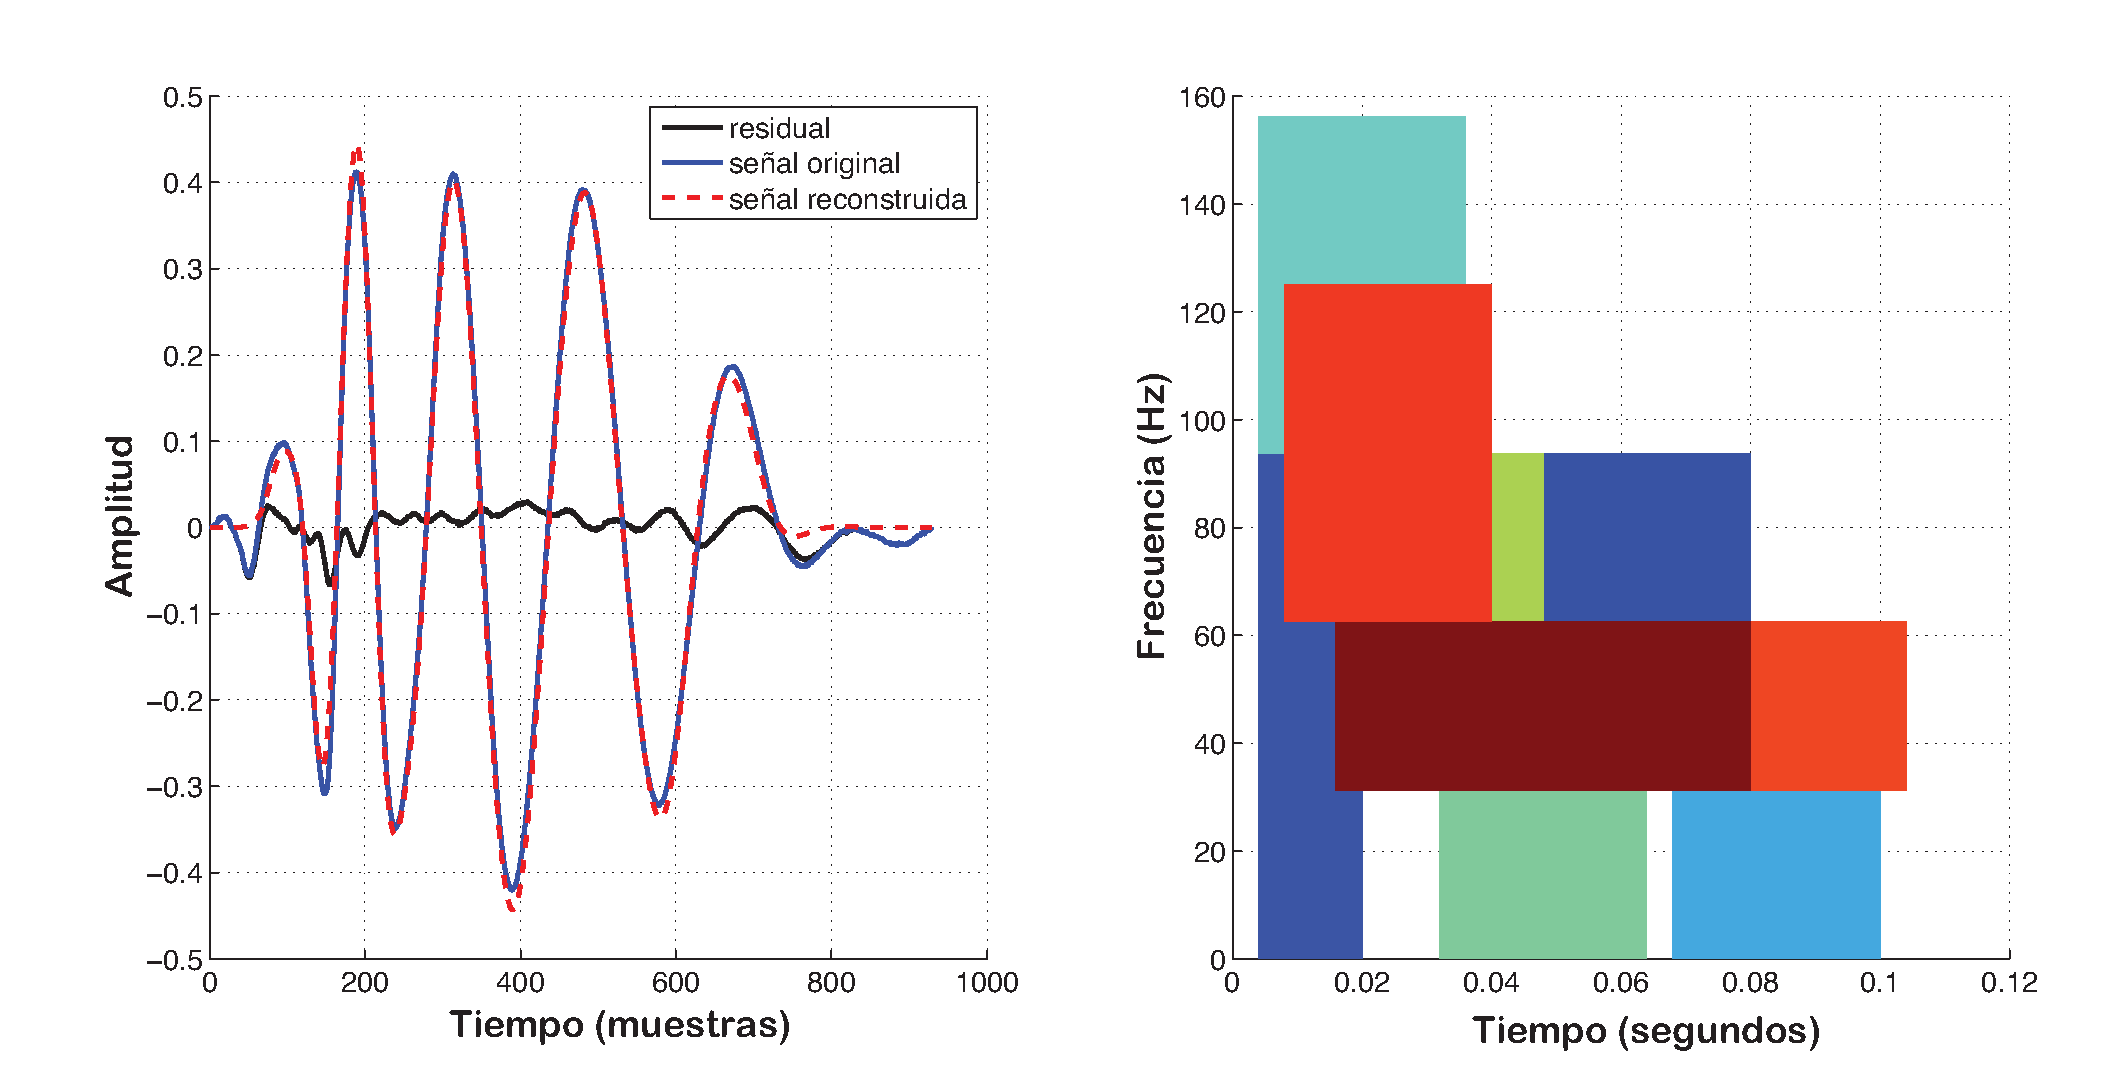
\includegraphics[scale=0.3]{eventoRecons.eps}
	\end{figure}
\end{frame}

\begin{frame}{Se\~nal residual}
	\begin{itemize}
		\item<2-> MP es un algoritmo \emph{codicioso} $\Rightarrow$ extrae la mayor cantidad de energ\'ia/informaci\'on de la se\~nal a representar.
		\item<3-> No existe un n\'umero l\'imite de $K$ iteraciones/\'atomos para detener el algoritmo, se requiere un criterio.
		\item<4-> En este trabajo se ha propuesto extraer 99\% de la energ\'ia contenida en los eventos o  bien llegar hasta 30 iteraciones.
		\item<5-> El 1\% restante es considerado, junto con los silencios, \alert{\emph{parte estoc\'astica}} del c\'odec.
			\begin{itemize}
				\item<6-> Baja correlaci\'on con los \'atomos de Gabor.
				\item<7-> No contiene propiedades determin\'isticas.
				\item<8-> A\'un contiene informaci\'on sobre el audio cardiaco.
			\end{itemize}
	\end{itemize} 
\end{frame}

\begin{frame}{Se\~nal residual}
El perfil de extracci\'on de energ\'ia dado por MP tiene un comportamiento asint\'otico.
	\begin{figure}
		\centering
		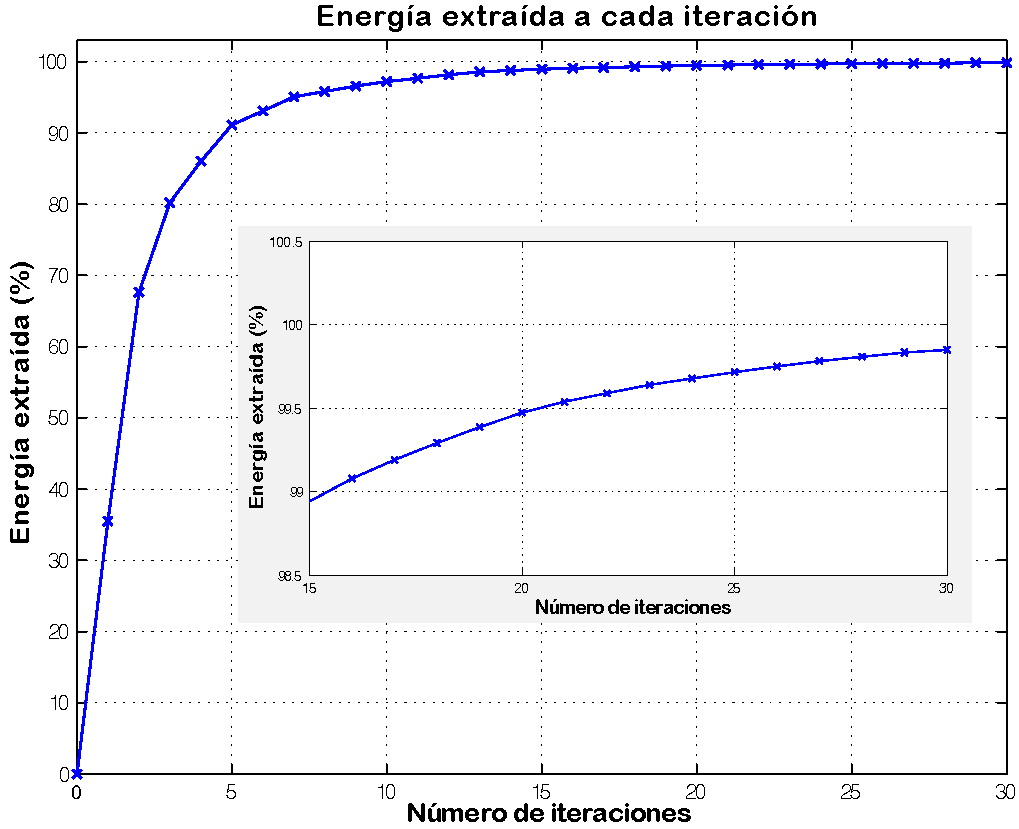
\includegraphics[scale=0.4]{perfil_energia_extraida.pdf}
	\end{figure}		
\end{frame}
%-------------------------------------------------------------------------------
%-------------------------------------------------------------------------------
% ,__ __                   _
%/|  |  |          |      | |          |
% |  |  |   __   __|   _  | |  __,   __|   __       _   __,   ,_  _|_  _
% |  |  |  /  \_/  |  |/  |/  /  |  /  |  /  \_   |/ \_/  |  /  |  |  |/
% |  |  |_/\__/ \_/|_/|__/|__/\_/|_/\_/|_/\__/    |__/ \_/|_/   |_/|_/|__/
%                                                /|
%                                                \|
%
%                                  o
% _   , _|_  __   __   _/,   , _|_     __   __,
%|/  / \_|  /  \_/    /  |  / \_|  |  /    /  |
%|__/ \/ |_/\__/ \___/\_/|_/ \/ |_/|_/\___/\_/|_/
%-------------------------------------------------------------------------------
%-------------------------------------------------------------------------------
\section{Modelado de la parte estoc\'astica}
% ----------------------------------------------------------------------
\begin{frame}{Se\~nal residual m\'as silencios}
El residual es obtenido al extraer en MP el 99\% de la energ\'ia de la se\~nal en las partes donde hubo eventos.
	\begin{figure}
		\centering
		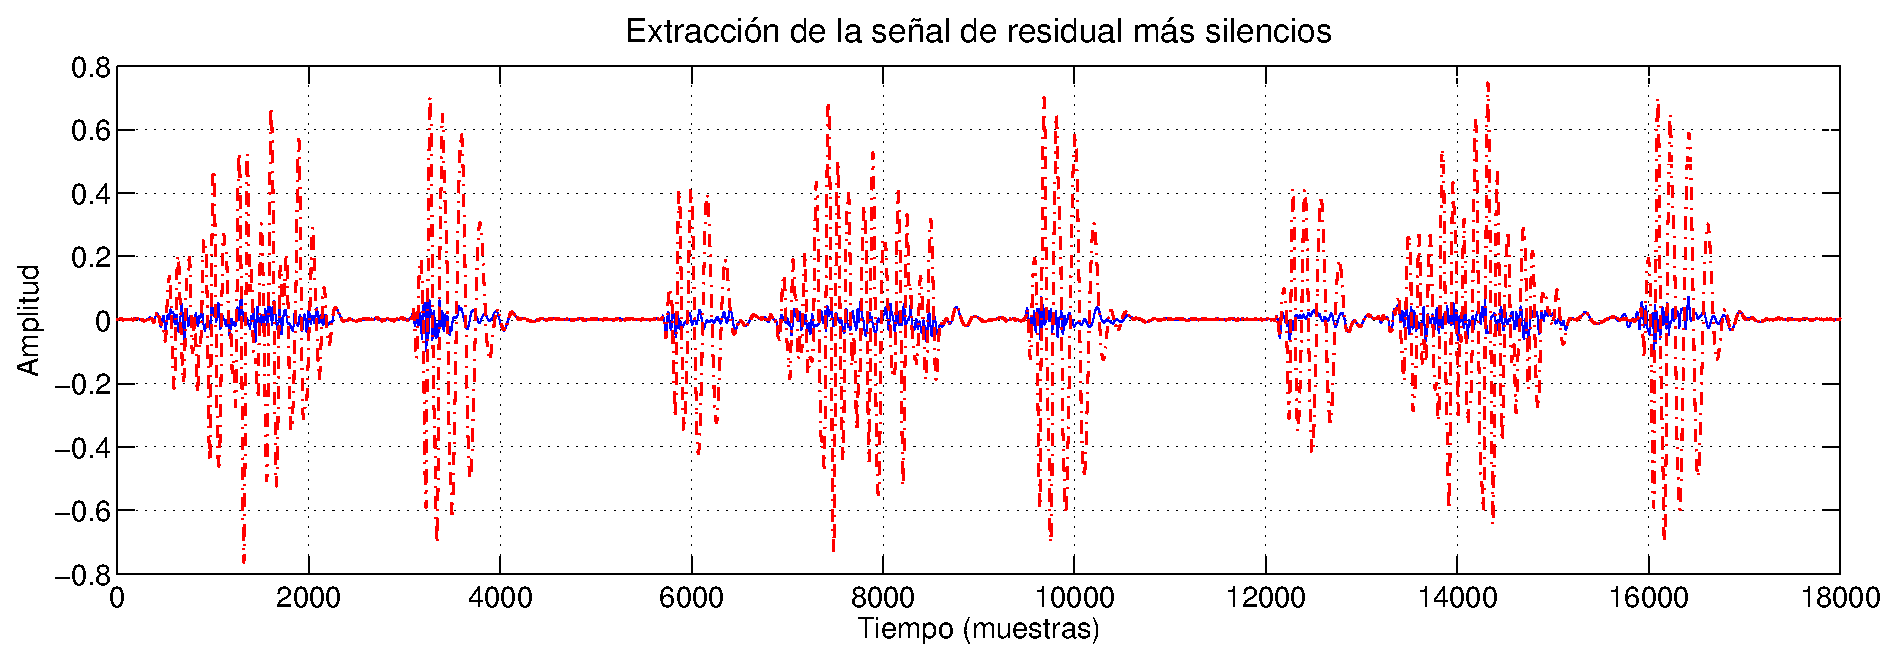
\includegraphics[scale=0.35]{extraccion_residual.eps}
	\end{figure}
\end{frame}

\begin{frame}{Modelado de la parte estoc\'astica}
		\begin{exampleblock}{Codificaci\'on predictiva lineal (LPC)}
			Bajo la hip\'otesis que el residual $R_{K}(t)$ es un proceso estoc\'astico estacionario en sentido amplio, en ventanas 			cortas de tiempo ($\approx 30$ ms) $s(n)$, puede ser generado por una ecuaci\'on en diferencias recursiva:
			$$ s(n) = \sum_{k=1}^{p}a_{k} s(n-k) + Gu(n),$$
			donde $a_{k}$ son los coeficientes de un filtro \emph{predictor}, $G$ es la ganancia del filtro y $s(n-k)$ son las $p$ muestras anteriores de $s(n)$.
		\end{exampleblock}
		Este modelo \alert{\emph{no pretende representar la forma de onda}}, sino aproximar la envolvente del espectro de la se\~nal $s(n)$.
\end{frame}


\begin{frame}{Modelo de predicci\'on lineal}
	La secuencia $s(n)$ se genera por medio de la excitaci\'on de un filtro IIR \emph{todo polos} mediante $u(n)$ teniendo dos casos:
	\begin{itemize}
		\item<2-> Sonido vocalizado (voiced): Se elige a $u(n)$ como un tren de pulsos separados por un \emph{periodo tonal} (pitch).
		\item<3-> Sonido no vocalizado (unvoiced): $u(n)$ es una secuencia de ruido gaussiano.
	\end{itemize}\pause
	\begin{figure}
		\centering
		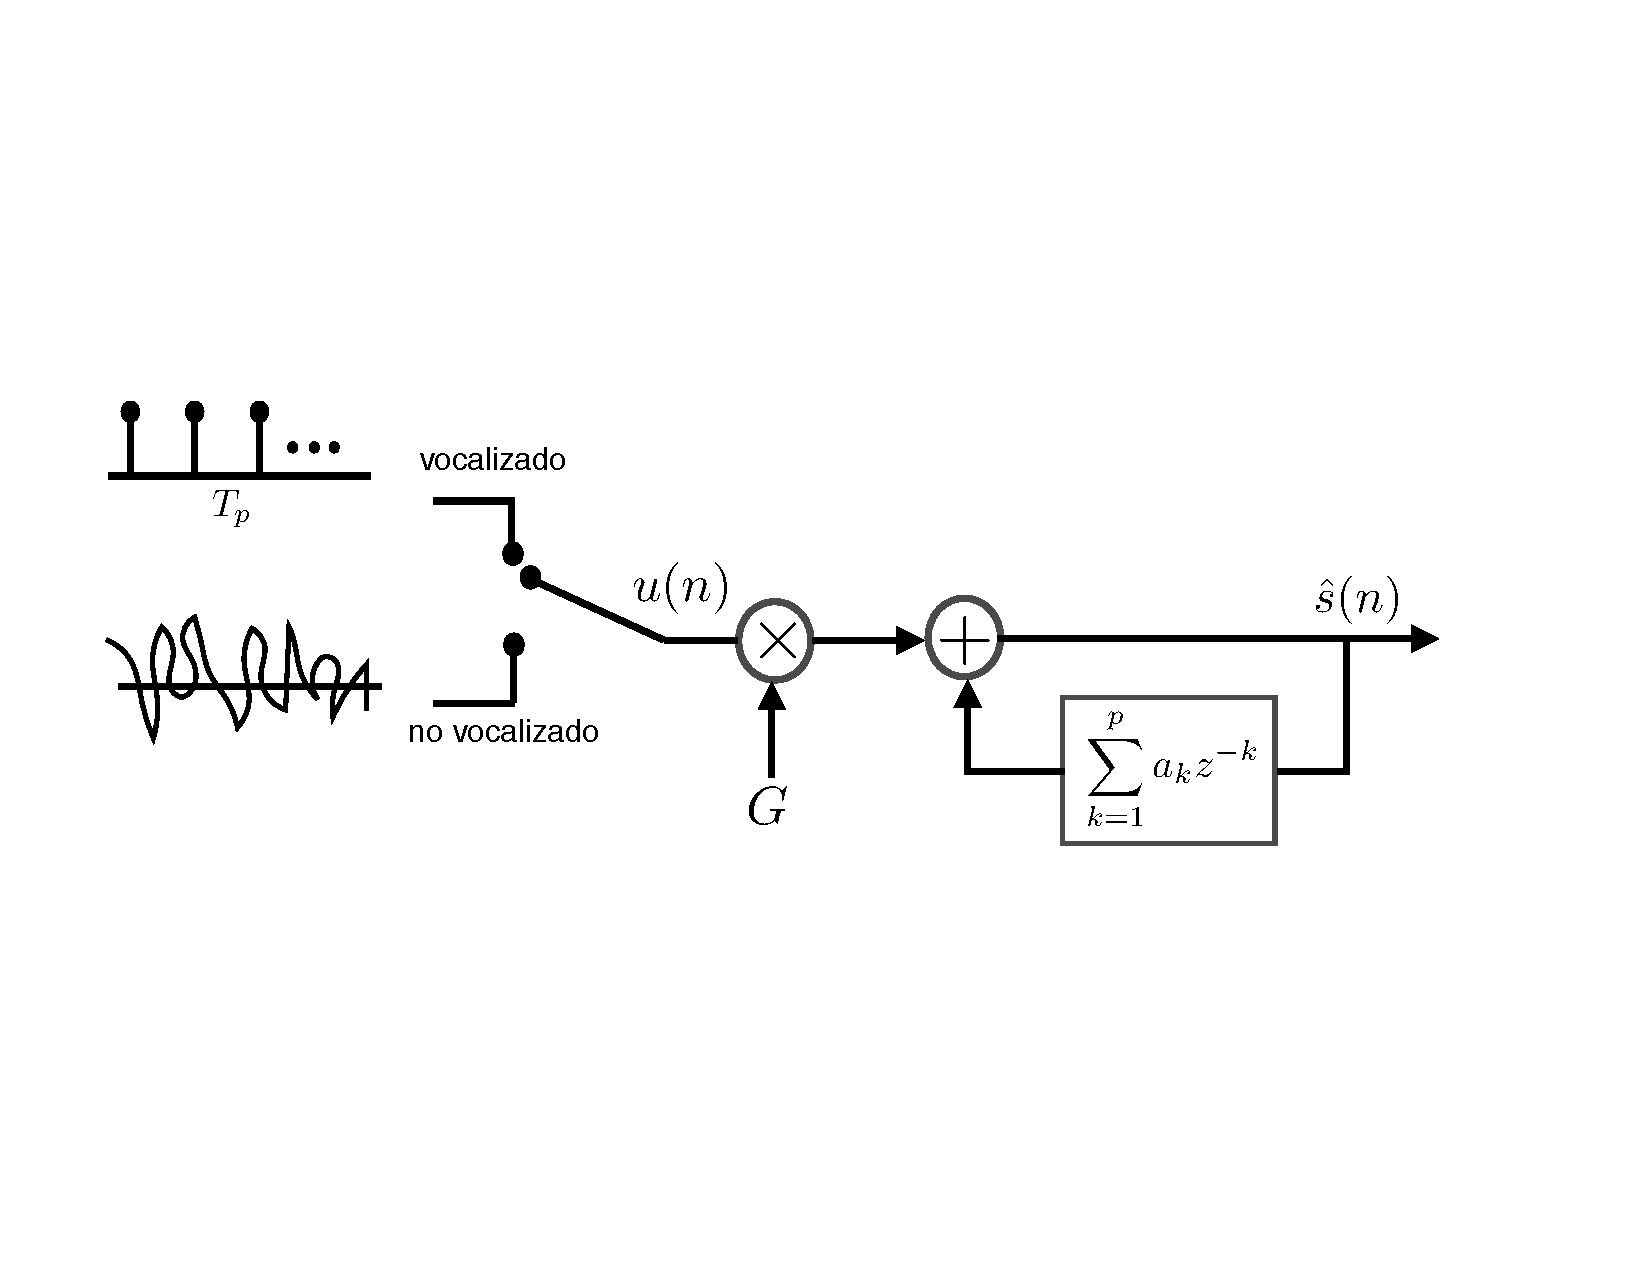
\includegraphics[scale=0.4]{lpc_syn.pdf}
	\end{figure}
\end{frame}

\begin{frame}{Modelado LPC de la parte estoc\'astica}
	Se divide la se\~nal residual m\'as silencios en ventanas de 256 muestras (32 ms si $fs=8$kHz) con un recubrimiento (overlap) del 50\% y se calcula para cada una de ellas los coeficientes predictores (recursi\'on de Levinson), y periodo tonal (caso vocalizado).
	\begin{figure}
		\centering
		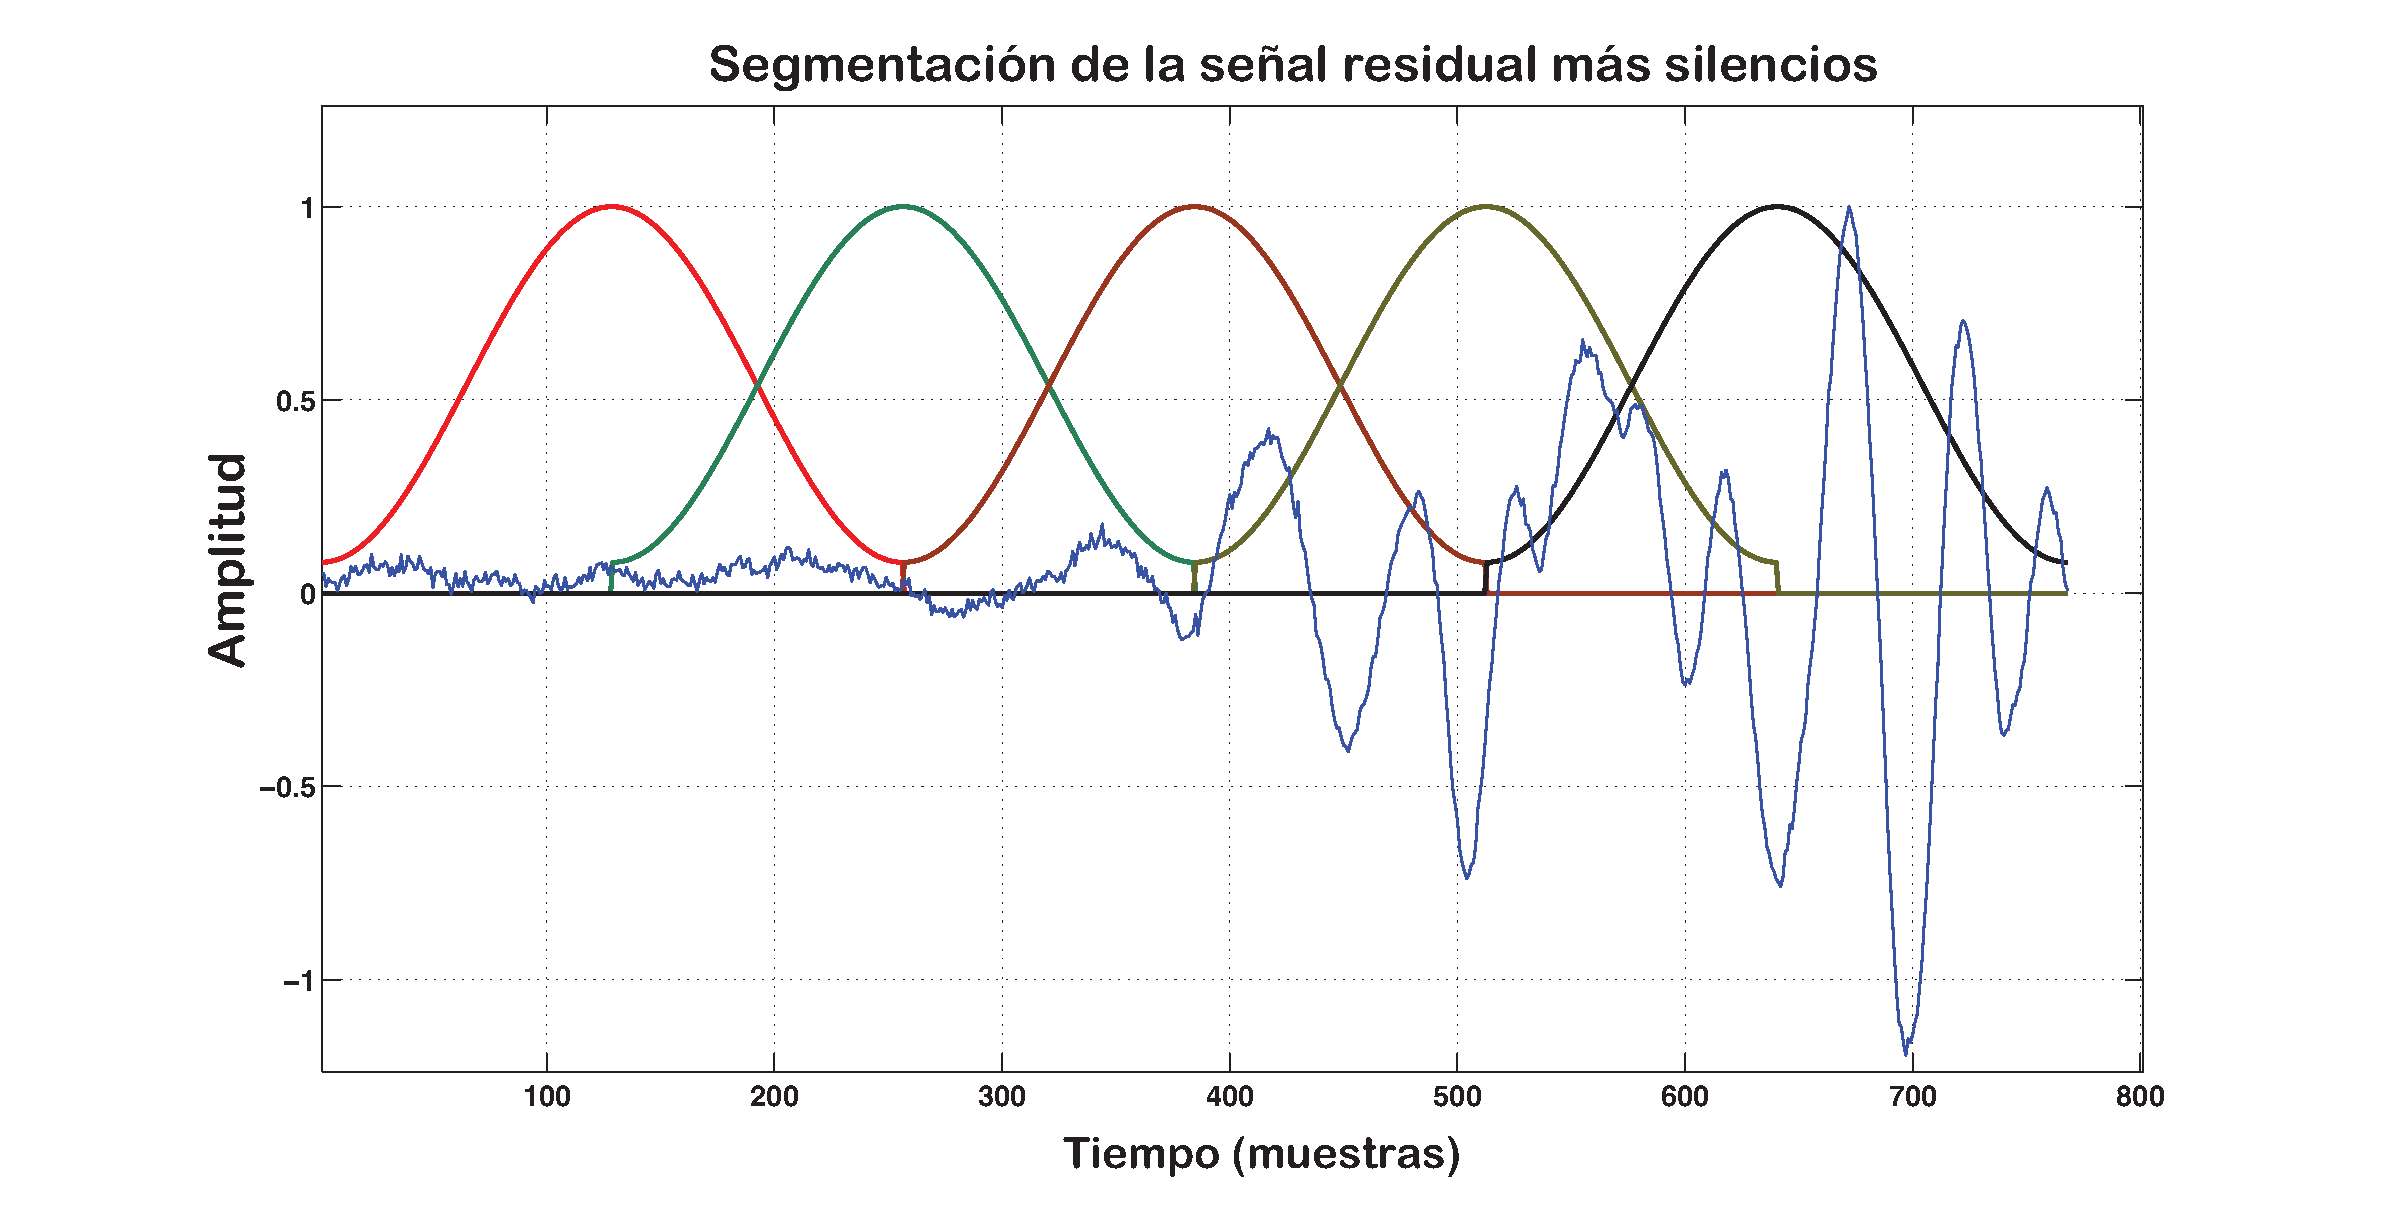
\includegraphics[scale=0.25]{OLA_plot.eps}
	\end{figure}
\end{frame}

\begin{frame}{Selecci\'on del orden del filtro}
	Se emple\'o la \emph{planitud espectral\footnote{Raz\'on entre la media geom\'etrica y media aritm\'etica de la PSD de la se\~nal.}} $\gamma_{x}^{2}$ promedio de las se\~nales analizadas para observar en su gr\'afica el punto donde el espectro comienza a comportarse como plano, teniendo en este caso $p=15$ y $p=10$.
	\begin{figure}
		\centering
		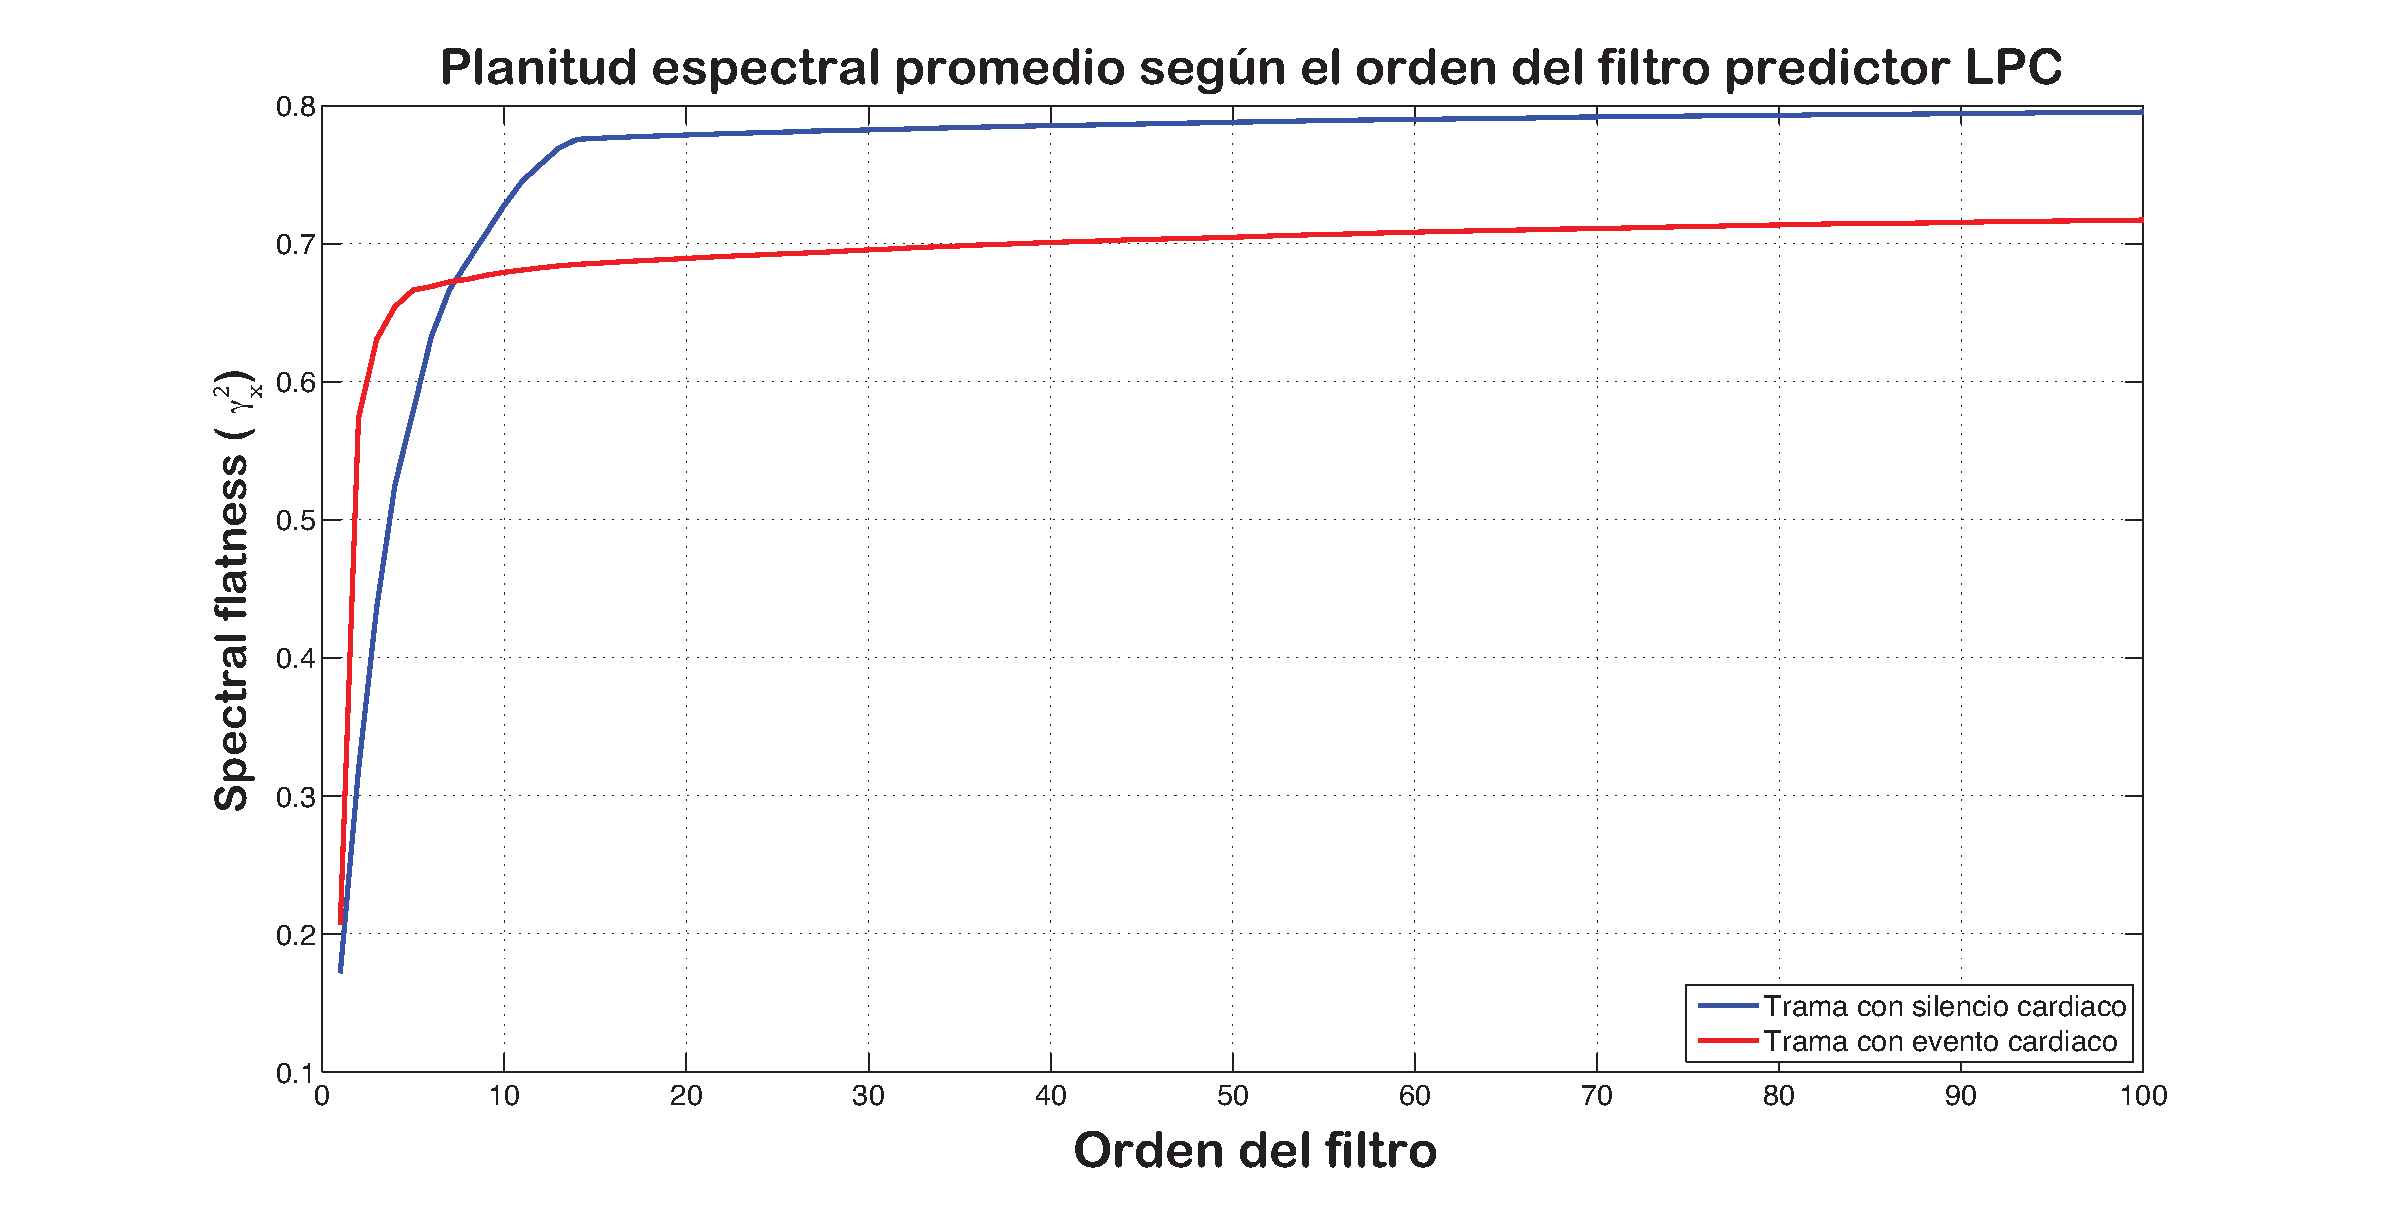
\includegraphics[scale=0.22]{sfm.eps}
	\end{figure}	
\end{frame}
%-------------------------------------------------------------------------------
%-------------------------------------------------------------------------------
% ___
%/ (_)                              o
%\__      _|_  ,_    __,   __   __      _/   _  _
%/    /\/  |  /  |  /  |  /    /    |  /  \_/ |/ |    |   |
%\___/ /\_/|_/   |_/\_/|_/\___/\___/|_/\__/   |  |_/   \_/|/
%                                                        /|
%                                                        \|
%                                 _
%                             o  | | o                  o
% __          __,   _  _  _|_    | |     __   __,   __      _/   _  _
%/    |   |  /  |  / |/ |  |  |  |/  |  /    /  |  /    |  /  \_/ |/ |
%\___/ \_/|_/\_/|_/  |  |_/|_/|_/|__/|_/\___/\_/|_/\___/|_/\__/   |  |_/
%                                |\
%                                |/
%             _
%   |        | |
% __|   _    | |  __   ,
%/  |  |/    |/  /  \_/ \_
%\_/|_/|__/  |__/\__/  \/
%
%
%   _   __,   ,_    _/   _  _  _    _ _|_  ,_    __   ,
% |/ \_/  |  /  |  /  |  / |/ |/ |  |/  |  /  |  /  \_/ \_
% |__/ \_/|_/   |_/\_/|_/  |  |  |_/|__/|_/   |_/\__/  \/
%/|
%\|
%-------------------------------------------------------------------------------
%-------------------------------------------------------------------------------
\section{Extracci\'on y cuantificaci\'on de los par\'ametros}
%-------------------------------------------------------------------------------
\begin{frame}{Cuantificaci\'on}
	\begin{itemize}
		\item<2-> Los valores de amplitud de una se\~nal toman valores discretos en la cuantificaci\'on.
		\item<3-> El proceso es irreversible y de compresi\'on con p\'erdidas.
		\item<4-> Matem\'aticamente equivale a a\~nadir ruido aditivo a la se\~nal.
	\end{itemize}\pause
	\begin{figure}
		\centering
		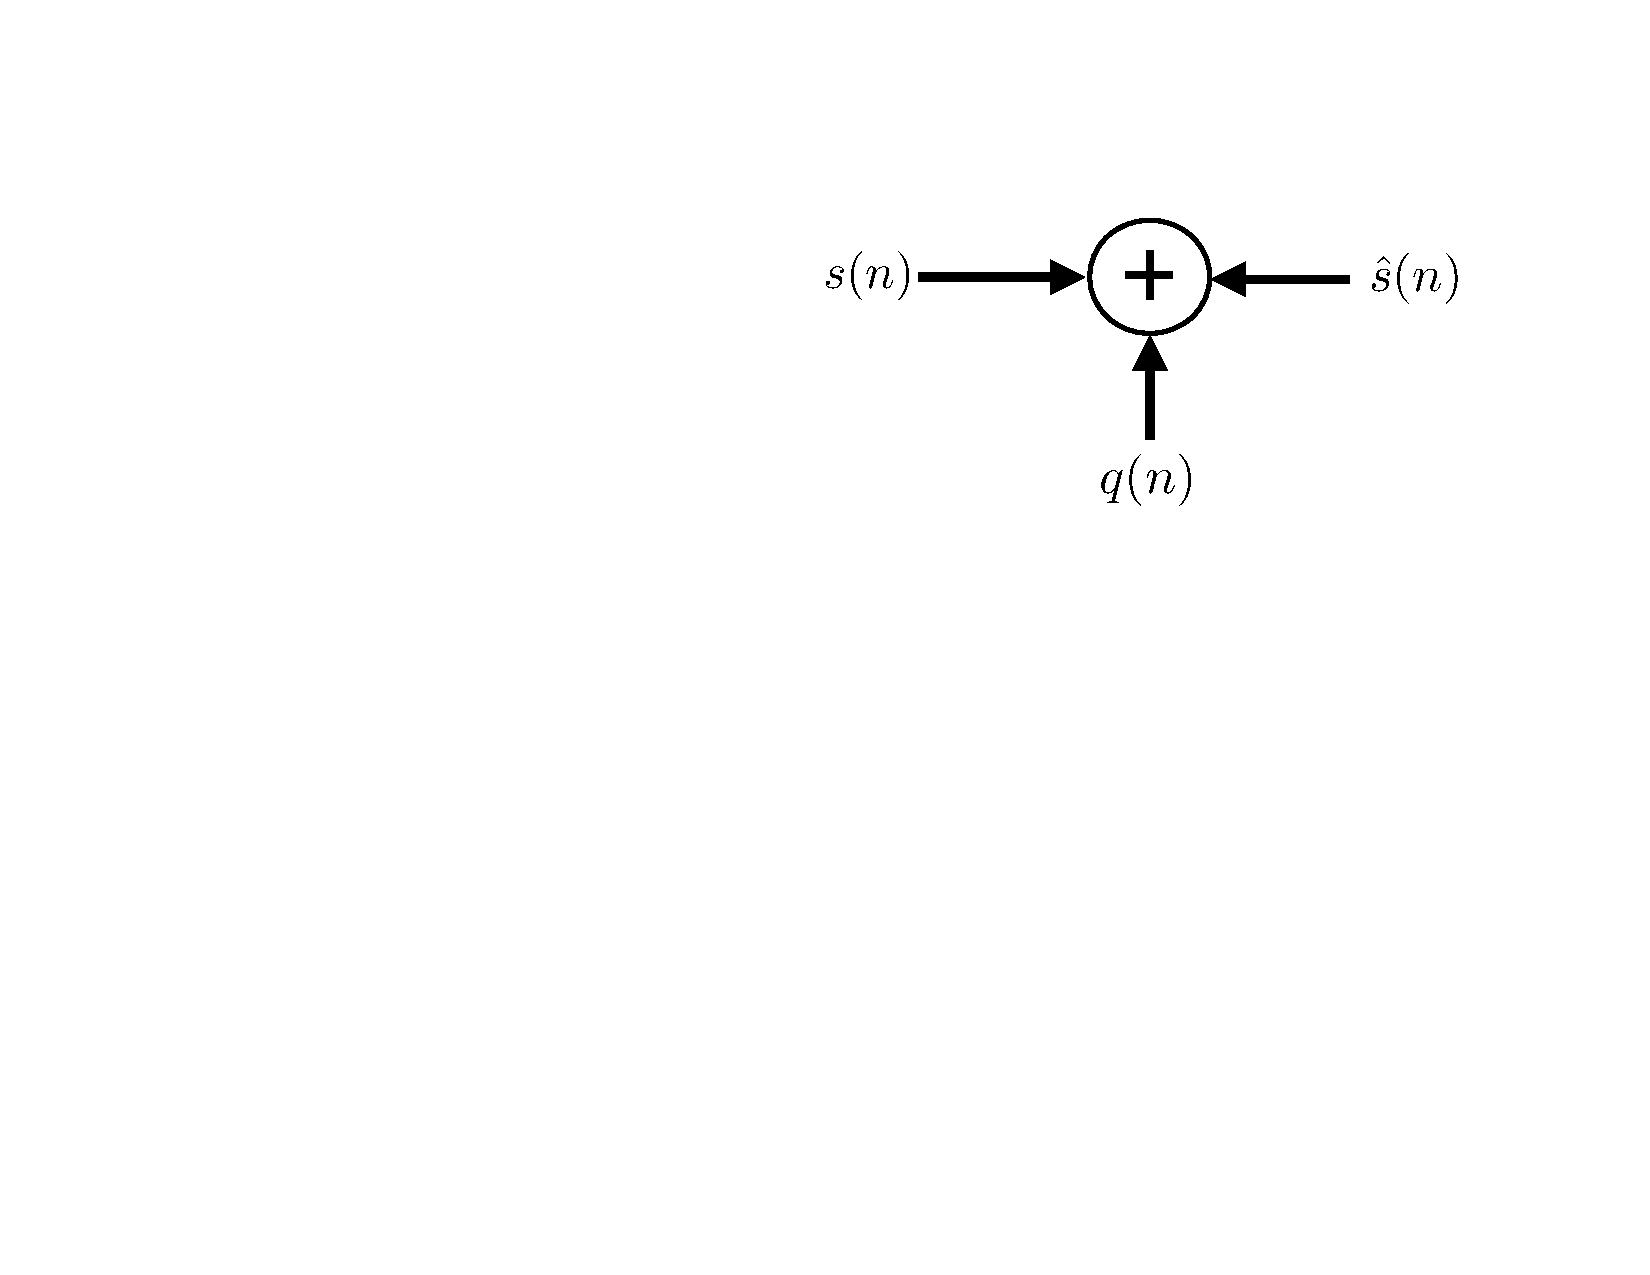
\includegraphics[width=0.6\textwidth]{quant2.pdf}
	\end{figure}
\end{frame}
\begin{frame}{Par\'ametros obtenidos en los modelados}
Se cuantificaron los par\'ametros extra\'idos que no son de formato \emph{entero}.
	\begin{figure}
		\centering
		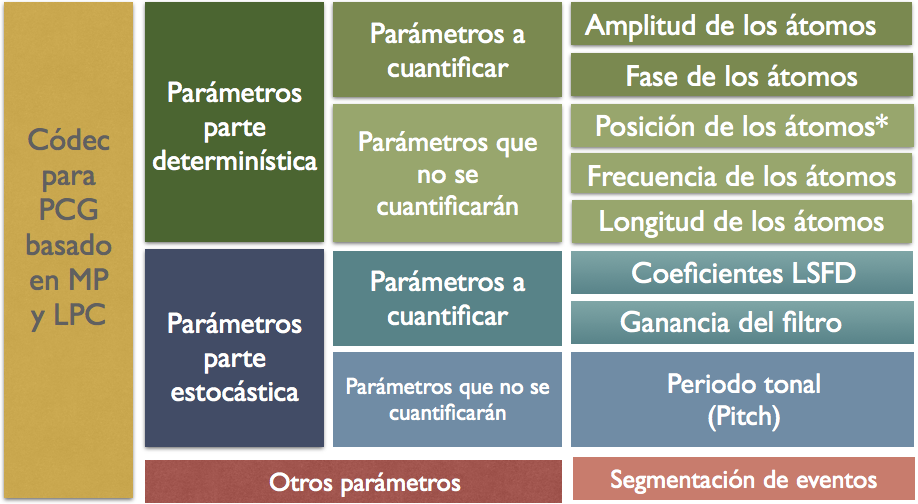
\includegraphics[scale=0.33]{params_cuant.png}
	\end{figure}
\end{frame}

\begin{frame}{Sensibilidad del filtro predictor}
	\begin{itemize}
		\item<2-> Varios de los polos del filtro predictor son muy cercanos al c\'irculo unitario. 
		\item<3-> No son directamente cuantificables, ya que no se preserva la \emph{estabilidad del filtro}.
	\end{itemize}\pause
	\begin{figure}
		\centering
		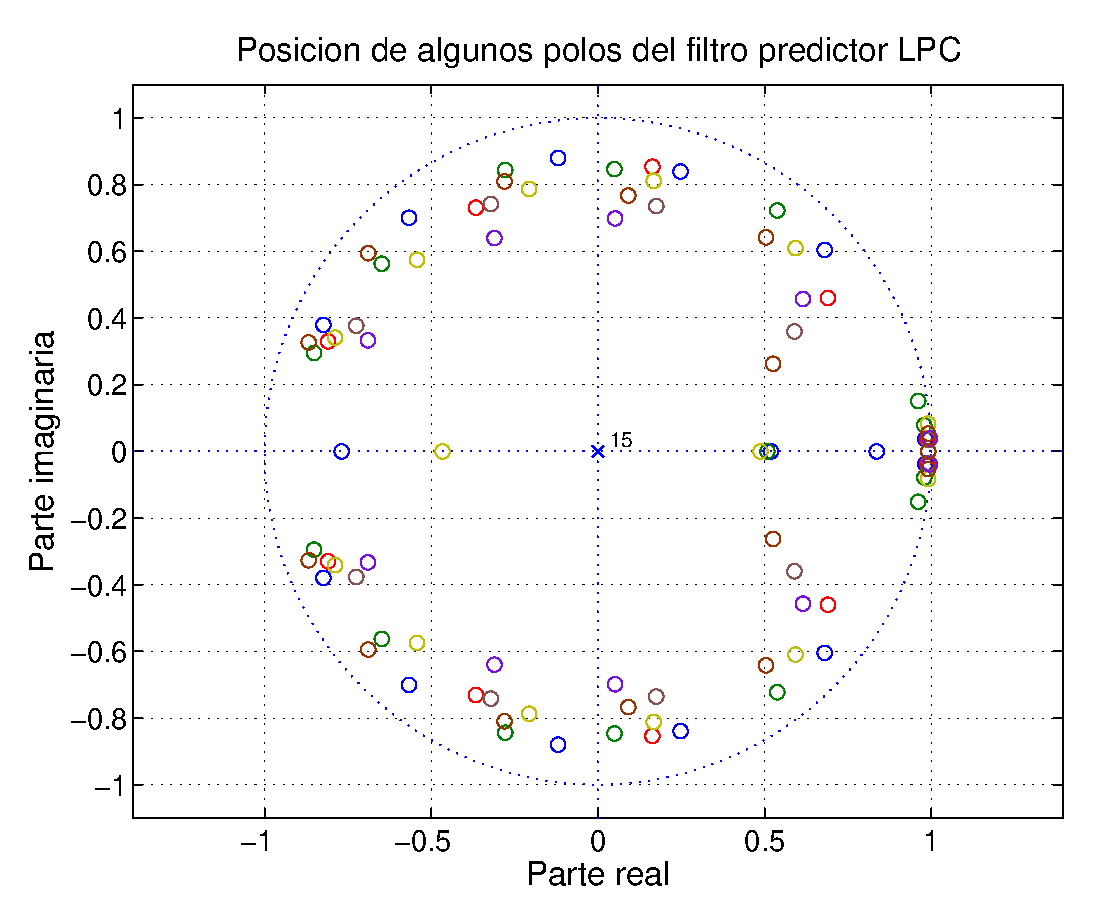
\includegraphics[scale=0.35]{polos_y_ceros.eps}
	\end{figure}	
\end{frame}

\begin{frame}{Distorsi\'on espectral com\'un}
	\begin{itemize}
		\item<2-> Existen otras representaciones equivalentes a los coeficientes predictores $a_{k}$.		
		\item<3-> Se ha calculado la \emph{distorsi\'on espectral com\'un} $D_{i}$ entre las tramas de audio cardiaco 				  reconstruidas tras cuantificar y las tramas originales.
	\end{itemize}
	\begin{figure}\pause
		\centering
		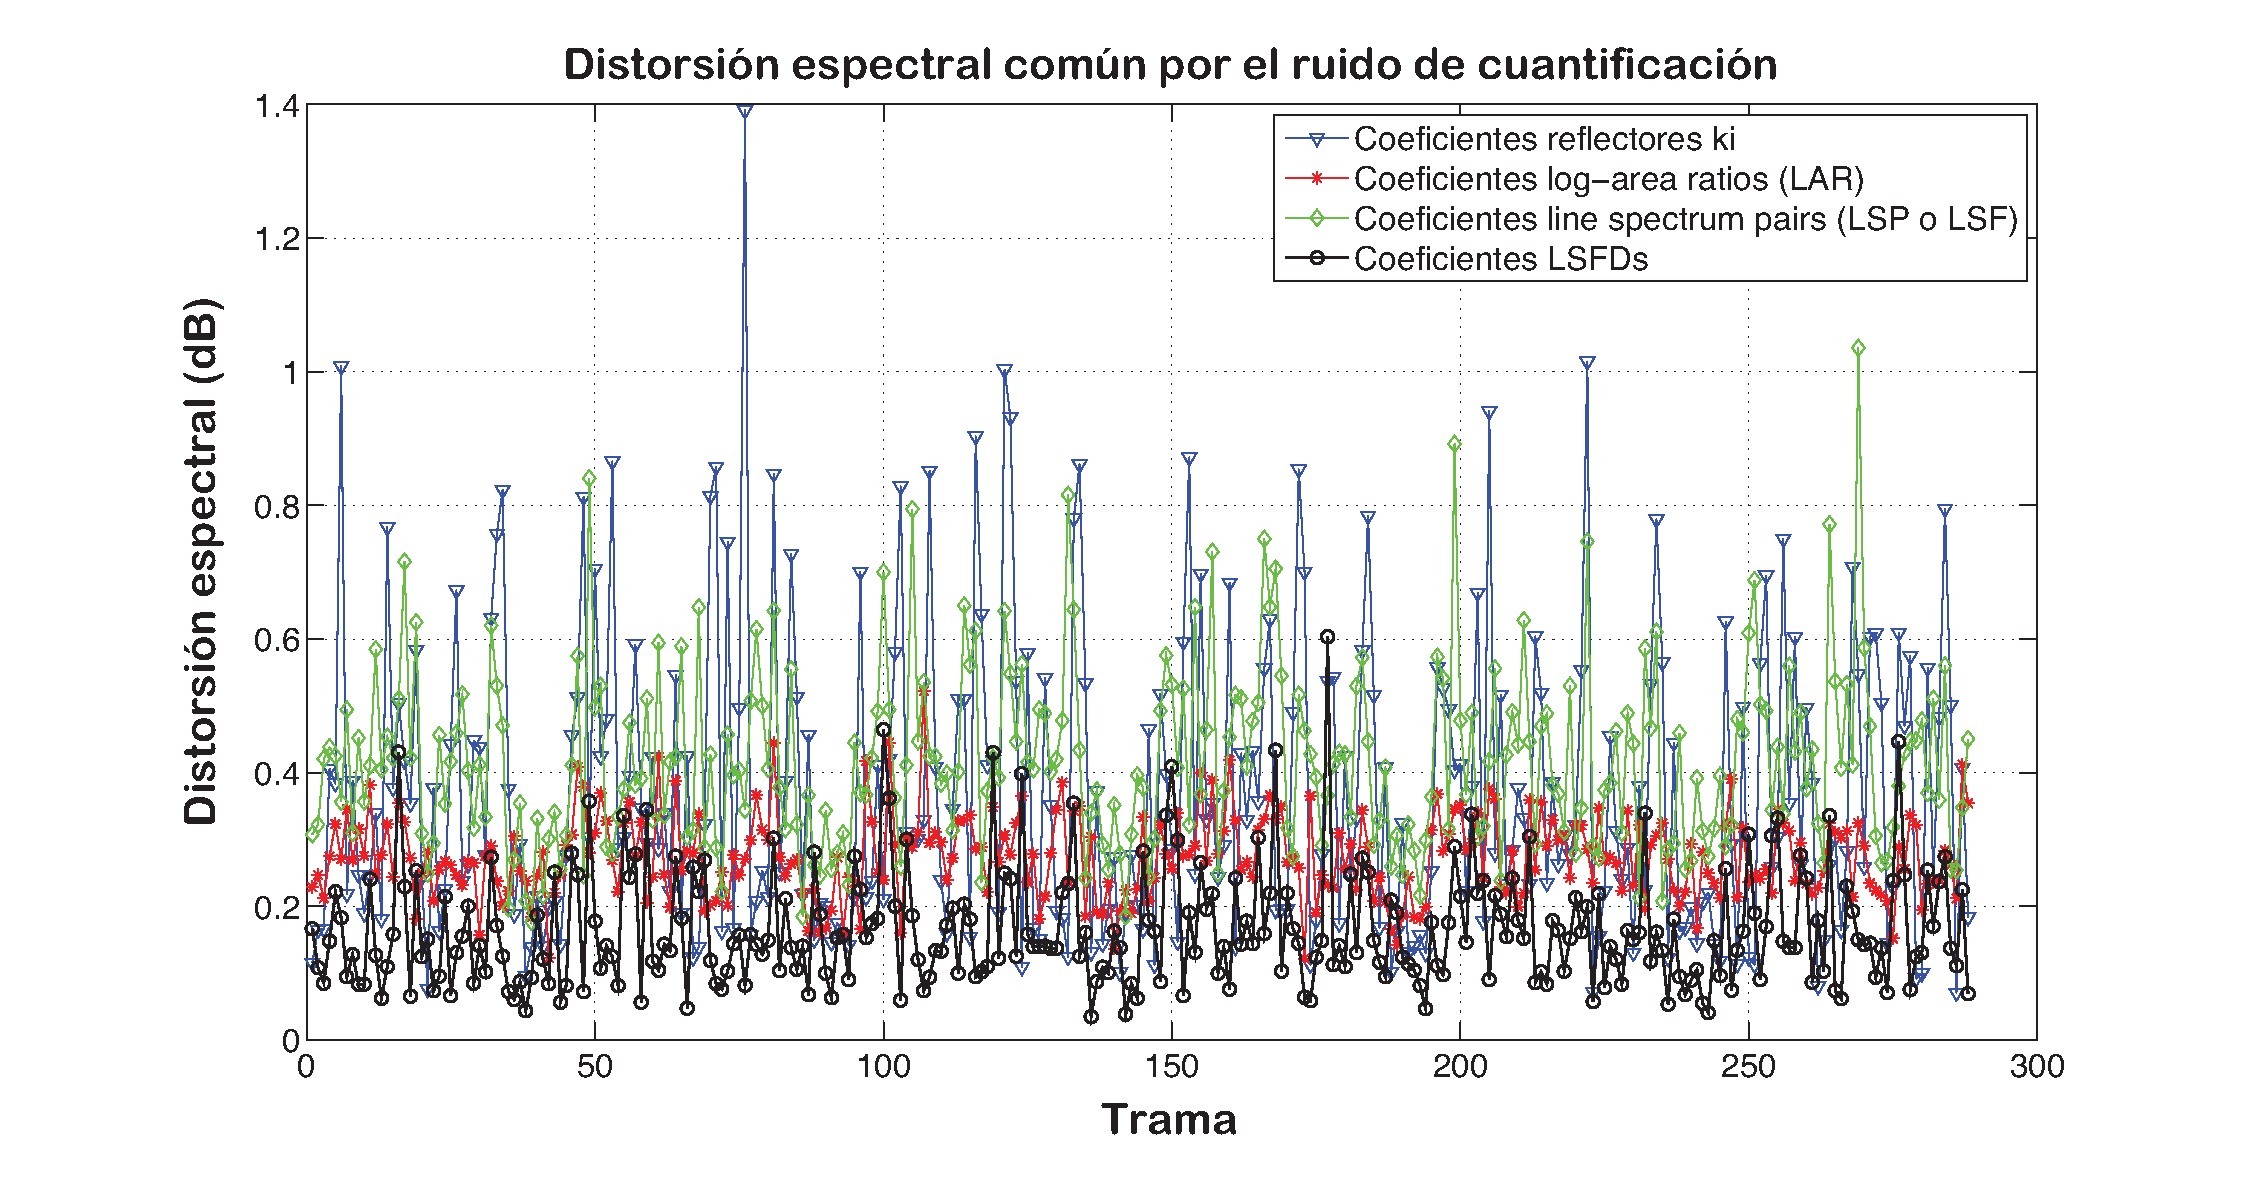
\includegraphics[scale=0.25]{spectral_disortion.eps}
	\end{figure}
\end{frame}
%-------------------------------------------------------------------------------
%-------------------------------------------------------------------------------
% ___             _
%/ (_)           | |                   o
%\__        __,  | |         __,   __      _/   _  _
%/    |  |_/  |  |/  |   |  /  |  /    |  /  \_/ |/ |    |   |
%\___/ \/  \_/|_/|__/ \_/|_/\_/|_/\___/|_/\__/   |  |_/   \_/|/
%                                                           /|
%                                                           \|
%                      _
%                     | |             |
% ,_    _   ,         | |_|_  __,   __|   __   ,
%/  |  |/  / \_|   |  |/  |  /  |  /  |  /  \_/ \_
%   |_/|__/ \/  \_/|_/|__/|_/\_/|_/\_/|_/\__/  \/
%-------------------------------------------------------------------------------
%-------------------------------------------------------------------------------
\section{Evaluaci\'on y resultados}
%-------------------------------------------------------------------------------
\begin{frame}{Reconstrucci\'on del PCG por el codificador}
	\begin{figure}
		\centering
		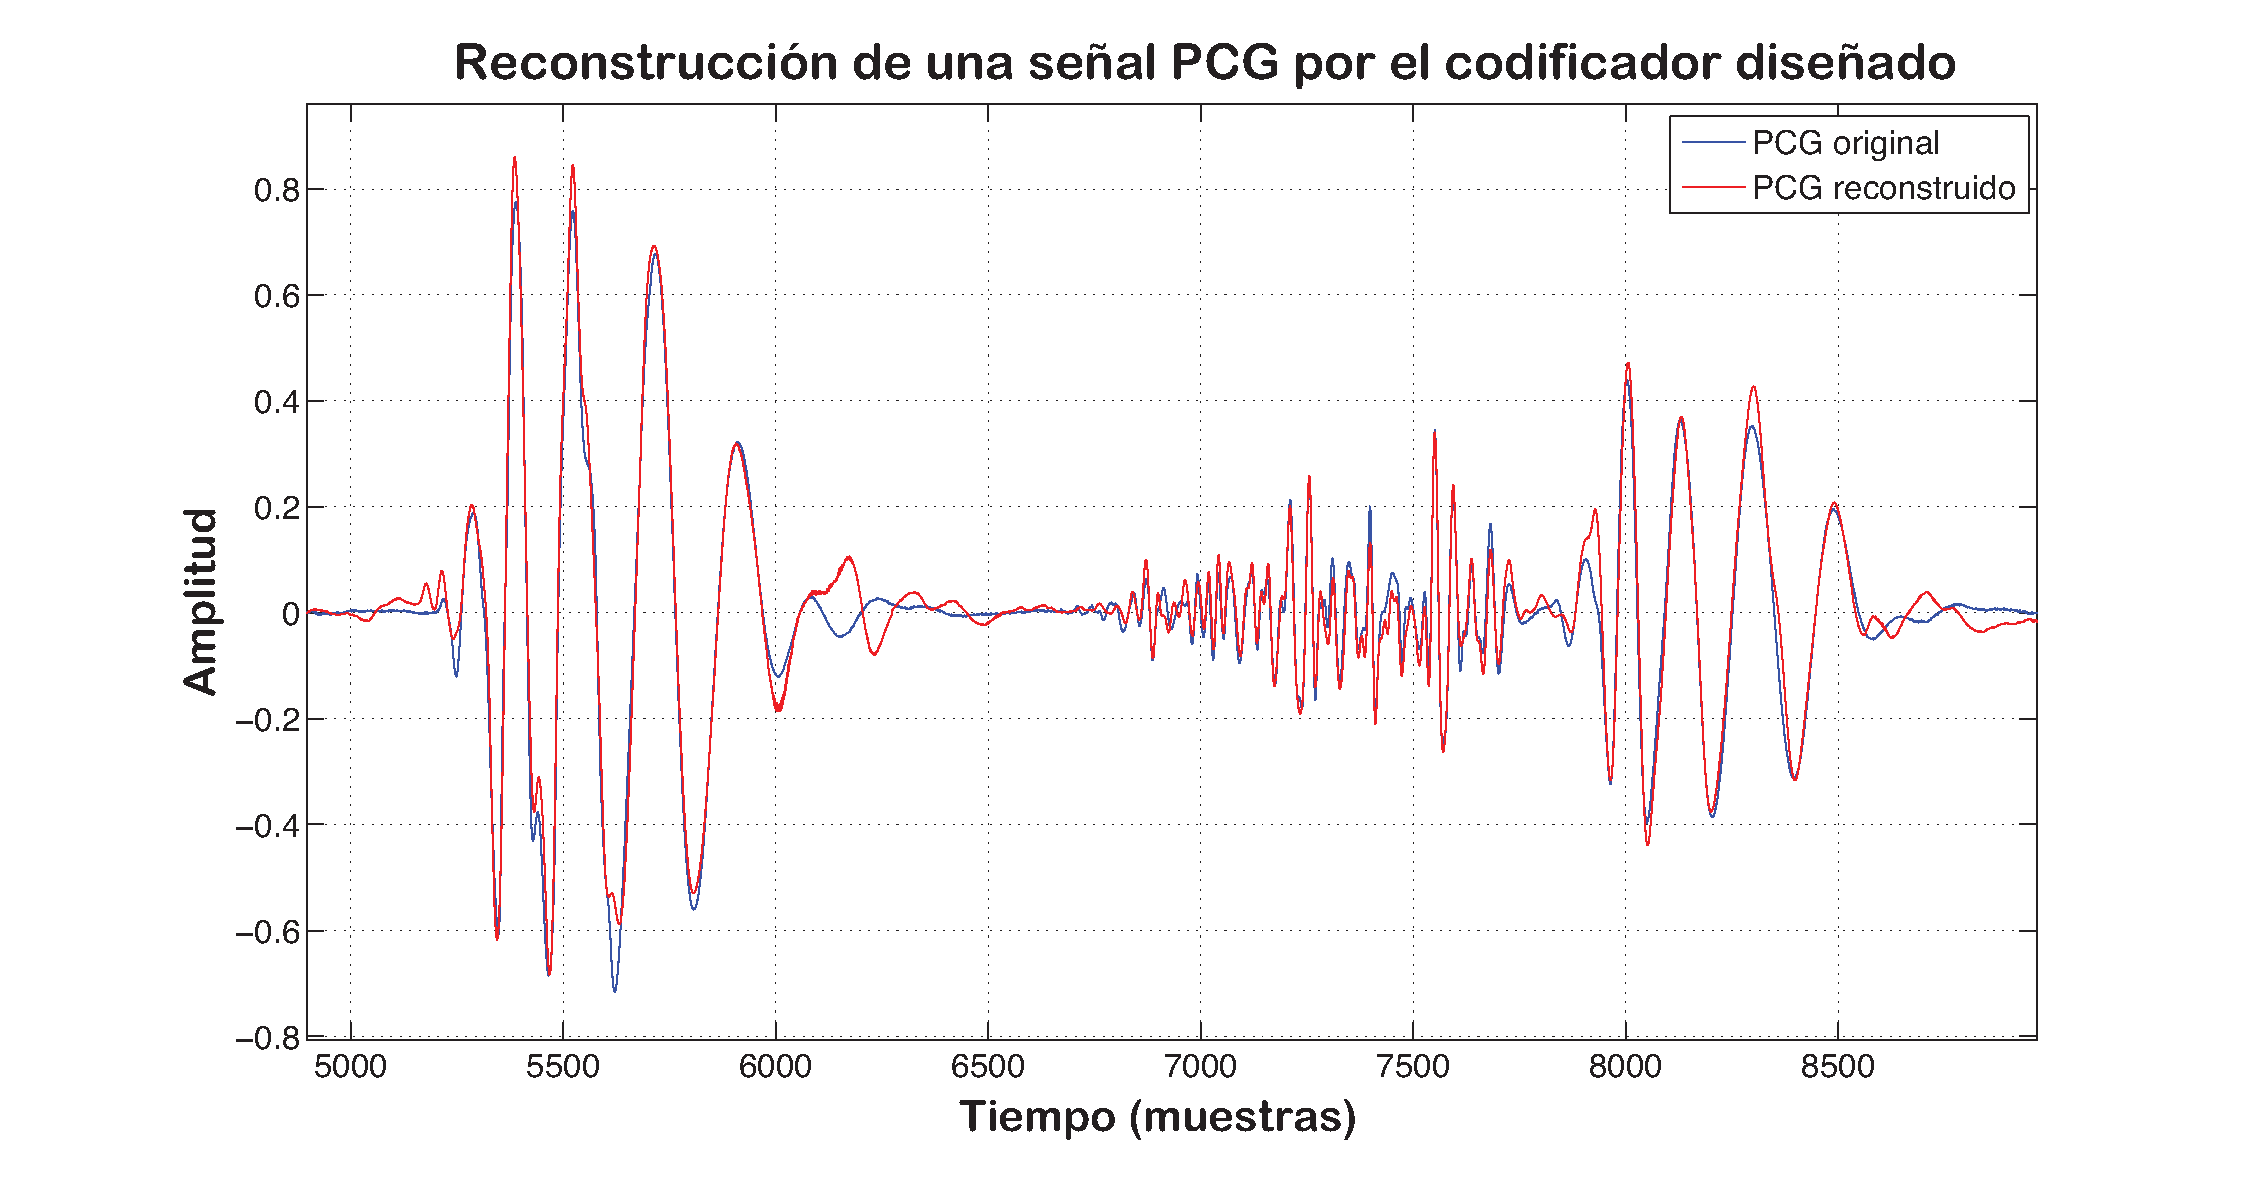
\includegraphics[scale=0.3]{pcgRecons.eps}
	\end{figure}
\end{frame}

\begin{frame}{Bits requeridos por par\'ametro}
	\begin{table}\scriptsize
		\centering
		\begin{tabular}{@{}lcl@{}}
		\toprule
		\multicolumn{3}{c}{Par\'ametros de la parte determin\'istica (MP)}                           \\ \midrule
	Par\'ametro extra\'ido    & \multicolumn{1}{l}{N\'um. bits requeridos/\'atomo} & Tipo de cuantificador \\ \midrule
		Amplitud at\'omica      & 8                                        & No uniforme           \\ \midrule
		Longitud at\'omica      & 3                                        & Sin cuantificador     \\ \midrule
		Fase at\'omica          & 8                                        & Uniforme              \\ \midrule
		Posici\'on at\'omica      & 8                                        & Sin cuantificador     \\ \midrule
		Frecuencia at\'omica    & 6                                        & Sin cuantificador     \\ \midrule
		\multicolumn{3}{c}{Par\'ametros de la parte estoc\'astica (LPC)}                            \\ \midrule
		Par\'ametro extra\'ido    & \multicolumn{1}{l}{N\'um. bits requeridos/segmento} & Tipo de cuantificador \\ \midrule
		Ganancia del filtro   & 4                                        & No uniforme           \\ \midrule
		Periodo tonal (Pitch) & 8                                        & Sin cuantificador     \\ \midrule
		LSFD                  & 7                                        & No uniforme          
		\end{tabular}
		\caption{N\'umero de bits requeridos por par\'ametro y tipo de cuantificaci\'on realizada.}
	\end{table}
\end{frame}

\begin{frame}{Porcentajes de compresi\'on en los PCG analizados}
\footnote{Se\~nales obtenidas de \url{http://solutions.3m.com.mx/wps/portal/3M/es_MX/3M-Littmann-LA/home/Education/SoundLibrary/}}
\begin{table}\scriptsize
\begin{tabular}{
>{\columncolor[HTML]{FFCCC9}}l 
>{\columncolor[HTML]{C3ECC1}}c 
>{\columncolor[HTML]{9CD49C}}c 
>{\columncolor[HTML]{A9E7F9}}c }
\hline
\multicolumn{1}{c}{\cellcolor[HTML]{C13333}{\color[HTML]{FFFFFF} }}                                              & \multicolumn{2}{c}{\cellcolor[HTML]{036400}{\color[HTML]{FFFFFF} \textbf{Porcentaje de compresi\'on (\%)}}}                                                         & \cellcolor[HTML]{3166FF}{\color[HTML]{FFFFFF} }                                                                                                         \\ \cline{2-3}
\multicolumn{1}{c}{\multirow{-2}{*}{\cellcolor[HTML]{C13333}{\color[HTML]{FFFFFF} \textbf{Nombre de la se\~nal}}}} & \multicolumn{1}{l}{\cellcolor[HTML]{80D564}{\color[HTML]{FFFFFF} @ 128 kbps}} & \multicolumn{1}{l}{\cellcolor[HTML]{2FB52F}{\color[HTML]{FFFFFF} @ 64 kbps}} & \multirow{-2}{*}{\cellcolor[HTML]{3166FF}{\color[HTML]{FFFFFF} \textbf{\begin{tabular}[c]{@{}c@{}}Bits requeridos \\ por el codificador\end{tabular}}}} \\ \cline{1-1} \cline{4-4} 
Soplo diast\'olico                                                                                                 & {\color[HTML]{000000} 93.24}                                                  & {\color[HTML]{000000} 86.47}                                                 & {\color[HTML]{000000} 39,818}                                                                                                                           \\ \hline
Clic de eyecci\'on                                                                                                 & {\color[HTML]{000000} 93.88}                                                  & {\color[HTML]{000000} 87.68}                                                 & {\color[HTML]{000000} 39,115}                                                                                                                           \\ \hline
Murmullo sist\'olico temprano                                                                                      & {\color[HTML]{000000} 93.35}                                                  & {\color[HTML]{000000} 86.70}                                                 & {\color[HTML]{000000} 43,301}                                                                                                                           \\ \hline
Murmullo sist\'olico tard\'io                                                                                        & {\color[HTML]{000000} 93.30}                                                  & {\color[HTML]{000000} 86.61}                                                 & {\color[HTML]{000000} 44,333}                                                                                                                           \\ \hline
Chasquido de apertura                                                                                            & {\color[HTML]{000000} 94.06}                                                  & {\color[HTML]{000000} 88.13}                                                 & {\color[HTML]{000000} 38,077}                                                                                                                           \\ \hline
S3                                                                                                               & {\color[HTML]{000000} 93.99}                                                  & {\color[HTML]{000000} 87.98}                                                 & {\color[HTML]{000000} 38,385}                                                                                                                           \\ \hline
S4                                                                                                               & {\color[HTML]{000000} 94.06}                                                  & {\color[HTML]{000000} 88.16}                                                 & {\color[HTML]{000000} 39,031}                                                                                                                           \\ \hline
Murmullo pansist\'olico                                                                                            & {\color[HTML]{000000} 93.00}                                                  & {\color[HTML]{000000} 86.00}                                                 & {\color[HTML]{000000} 47,358}                                                                                                                           \\ \hline
Apertura normal S1                                                                                               & {\color[HTML]{000000} 94.49}                                                  & {\color[HTML]{000000} 88.98}                                                 & {\color[HTML]{000000} 31,602}                                                                                                                           \\ \hline
Apertura normal S2                                                                                               & {\color[HTML]{000000} 94.21}                                                  & {\color[HTML]{000000} 88.43}                                                 & {\color[HTML]{000000} 34,005}                                                                                                                           \\ \hline
\end{tabular}
\end{table}
\end{frame}


\begin{frame}{Evaluaci\'on objetiva del c\'odec}
Se calcul\'o el coeficiente de correlaci\'on $\rho_{x,\hat{x}}$ y la ra\'iz cuadrada de la diferencia cuadr\'atica media (PRD) de las se\~nales analizadas:

\begin{table}\scriptsize
\begin{tabular}{
>{\columncolor[HTML]{ECF4FF}}l 
>{\columncolor[HTML]{FFCE93}}c 
>{\columncolor[HTML]{9AFF99}}c }
\hline
\multicolumn{1}{c}{\cellcolor[HTML]{00009B}{\color[HTML]{FFFFFF} \textbf{Nombre de la se\~nal}}} & \cellcolor[HTML]{9A0000}{\color[HTML]{FFFFFF} \textbf{\begin{tabular}[c]{@{}c@{}}Coeficiente\\ de \\ correlaci\'on\end{tabular}}} & \cellcolor[HTML]{009901}{\color[HTML]{FFFFFF} \textbf{PRD (\%)}} \\ \hline
Soplo diast\'olico                                                                               & 0.97                                                                                                                            & 2.50                                                        \\ \hline
Clic de eyecci\'on                                                                               & 0.97                                                                                                                            & 2.38                                                        \\ \hline
Murmullo sist\'olico temprano                                                                    & 0.97                                                                                                                            & 2.33                                                        \\ \hline
Murmullo sist\'olico tard\'io                                                                      & 0.93                                                                                                                            & 2.41                                                        \\ \hline
Chasquido de apertura                                                                          & 0.93                                                                                                                            & 2.15                                                        \\ \hline
S3                                                                                             & 0.94                                                                                                                            & 2.87                                                        \\ \hline
S4                                                                                             & 0.96                                                                                                                            & 2.77                                                        \\ \hline
Murmullo pansist\'olico                                                                          & 0.96                                                                                                                            & 2.74                                                        \\ \hline
Apertura normal S1                                                                             & 0.96                                                                                                                            & 2.77                                                        \\ \hline
Apertura normal S2                                                                             & 0.97                                                                                                                            & 2.61                                                        \\ \hline
\end{tabular}

\end{table}

\end{frame}

\begin{frame}{Evaluaci\'on subjetiva del c\'odec}
	\begin{itemize}
		\item<2-> Se aplic\'o la norma ITU-T BS-1534 MUSHRA\footnote{\tiny{Mutiple Stimuli with Hidden Reference and Anchor.}}.
		\item<3-> Se compar\'o el modelo propuesto con los codificadores OPUS y MP3. 
	\end{itemize}\pause	
	\begin{figure}
		\centering
		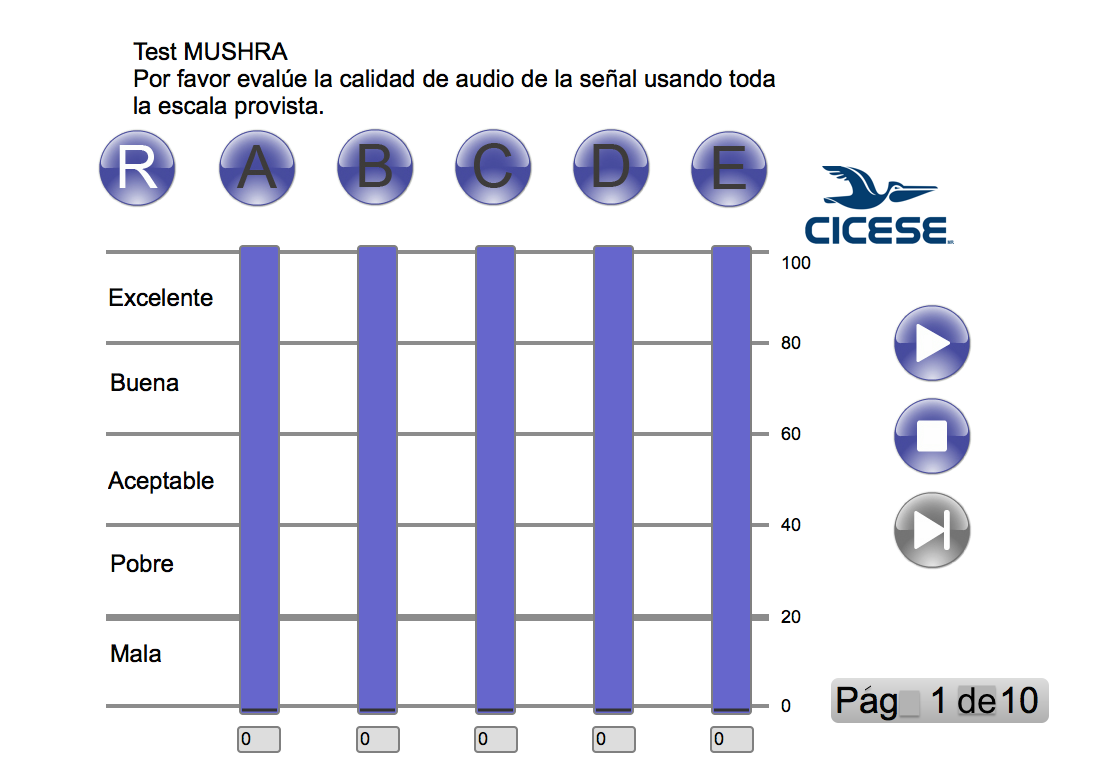
\includegraphics[scale=0.2]{mushra_interfaz.png}
	\end{figure}
\end{frame}

\begin{frame}{Resultados obtenidos por MUSHRA}
Se seleccionaron 5 est\'imulos para ser calificados, sus calificaciones promedio e intervalos de confianza para un nivel del 95\% fueron calculados. 
	\begin{figure}
		\centering
		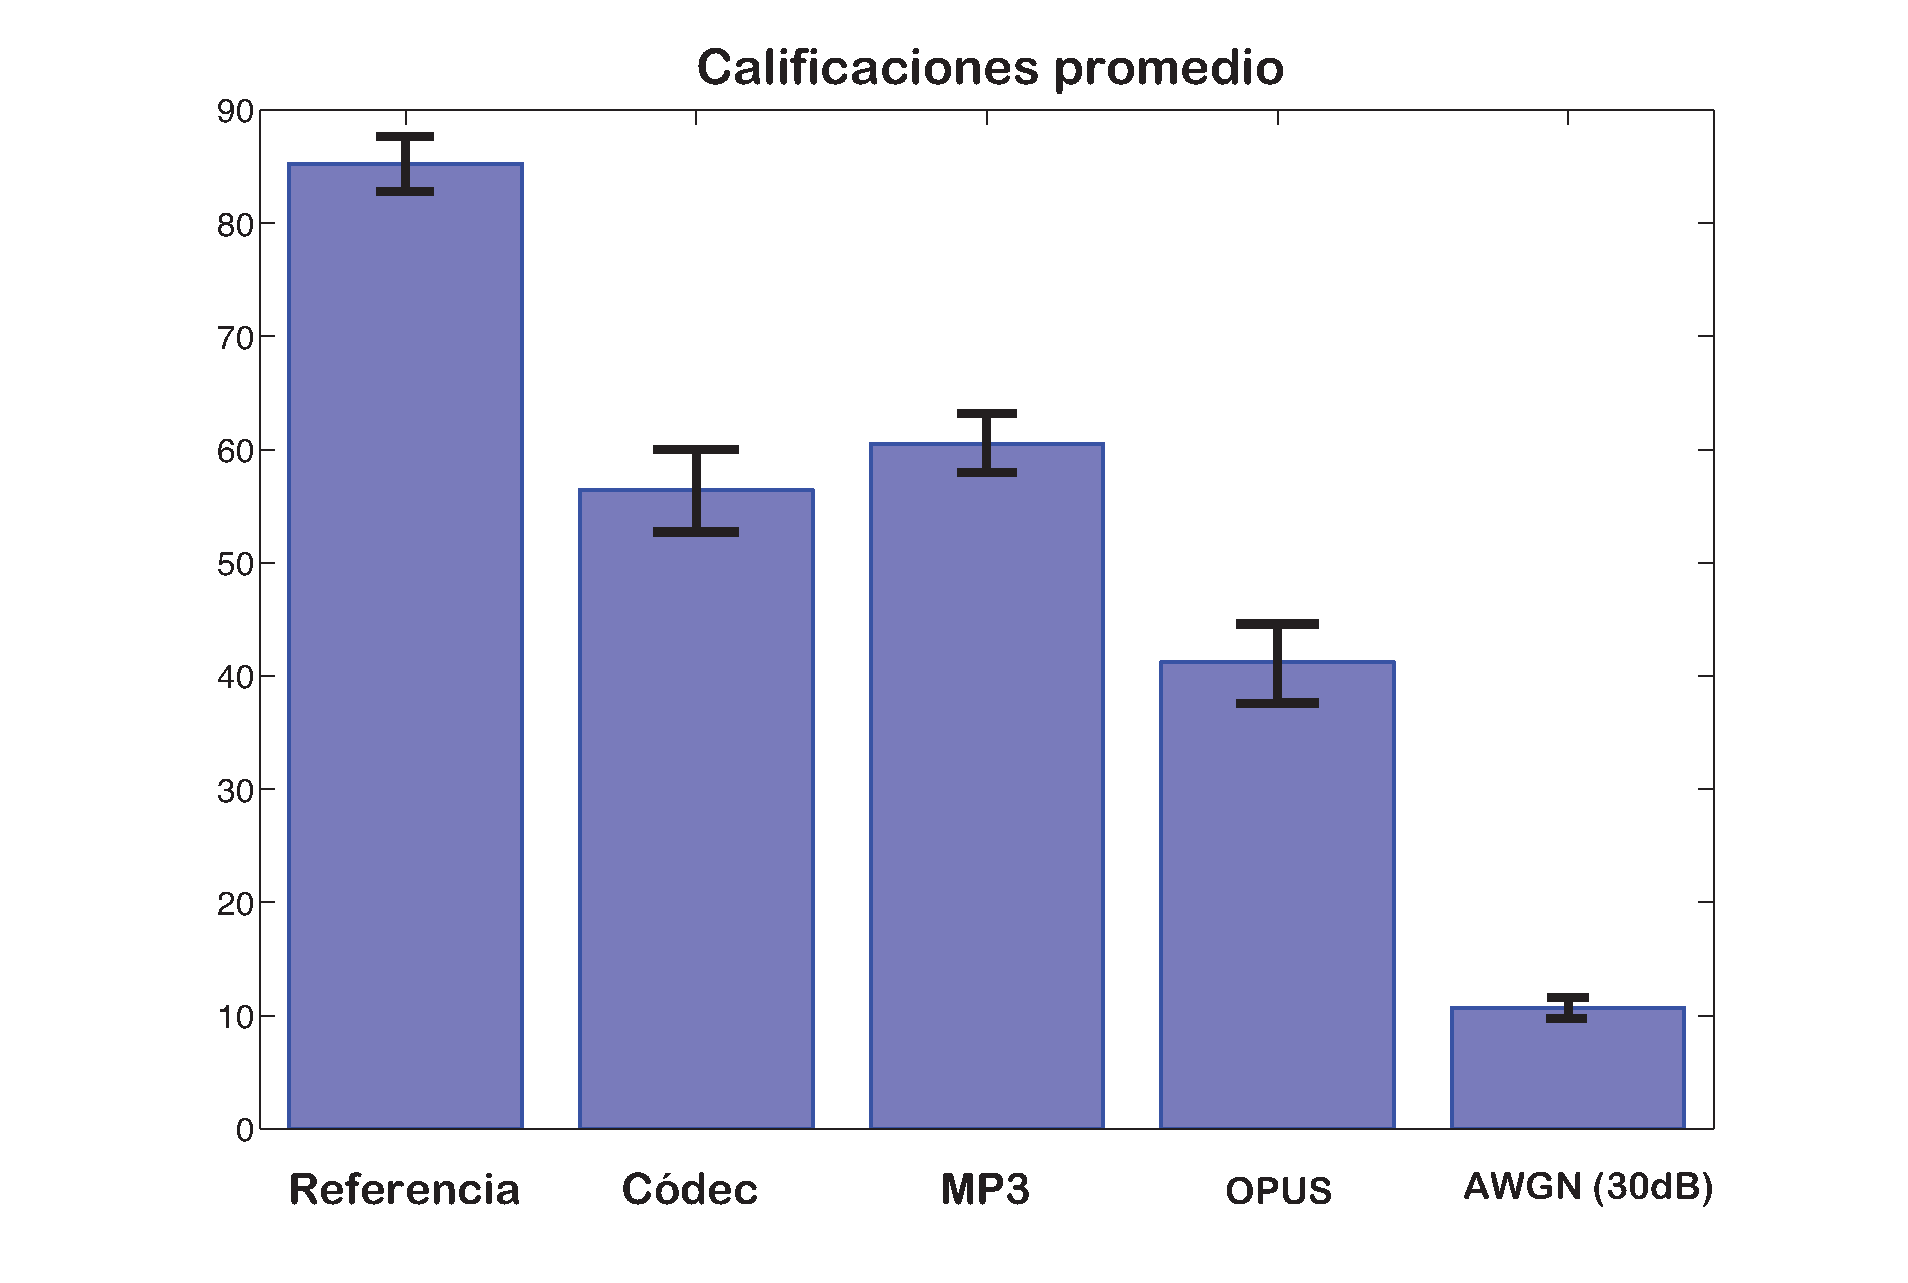
\includegraphics[scale=0.28]{CalifTotal.eps}
	\end{figure}
\end{frame}



%-------------------------------------------------------------------------------
%-------------------------------------------------------------------------------
%  ___                    _
% / (_)                  | |            o
%|      __   _  _    __  | |         ,      __   _  _    _   ,
%|     /  \_/ |/ |  /    |/  |   |  / \_|  /  \_/ |/ |  |/  / \_  |   |
% \___/\__/   |  |_/\___/|__/ \_/|_/ \/ |_/\__/   |  |_/|__/ \/    \_/|/
%                                                                    /|
%                                                                    \|
%                _                   _
%               | |        o        | |
%_|_  ,_    __, | |   __,     __    | |       _|_         ,_    __
% |  /  |  /  | |/ \_/  |  | /  \_  |/  |   |  |  |   |  /  |  /  \_
% |_/   |_/\_/|_/\_/ \_/|_/|/\__/   |__/ \_/|_/|_/ \_/|_/   |_/\__/
%                         /|        |\
%                         \|        |/
%-------------------------------------------------------------------------------
%-------------------------------------------------------------------------------
\section{Conclusiones y trabajo a futuro}
%-------------------------------------------------------------------------------
\begin{frame}{Conclusiones}
	\begin{itemize}
		\item<2-> Se desarroll\'o un codificador-decodificador para se\~nales de audio cardiaco $x(t)$ basado en la suma de una parte determin\'istica y una parte estoc\'astica:
		\[
 x(t) = \underbrace{\sum_{m}^K \alpha_{k}g_{\gamma_{m}}(t)}_{\text{parte determin\'istica}} + \underbrace{R_{K}(t)}_{\text{parte estoc\'astica}}
\].
	\item<3-> El codificador tiene una $R_{b}=8 $kbps y una tasa de compresi\'on $C_{r}\approx 94\%.$
	\item<4-> No se ha encontrado en la literatura un codificador con estas caracter\'isticas.
	\item<5-> Matching Pursuit y los diccionarios de Gabor reconstruyen con precisi\'on las partes del PCG correspondientes a eventos cardiacos.
	\end{itemize}
\end{frame}
\begin{frame}{Conclusiones}	
	\begin{itemize}
	\item<2-> La se\~nal residual $R_{K}(t)$ es a\'un perceptible e importante de modelar, su comportamiento se considera estoc\'astico por su baja correlaci\'on con los \'atomos (a pesar de ser el 1\% de la energ\'ia).
	\item<3-> Por medio de LPC fue posible modelar la parte estoc\'astica, segmentando la se\~nal en tramos de tiempo adecuados.
	\item<4-> Es importante la realizaci\'on de pruebas subjetivas en condiciones adecuadas para los oyentes.
	\item<5-> Los intervalos de confianza dan una valoraci\'on aceptable al codificador frente a versiones MP3 y OPUS, tomando adem\'as niveles del 95\% de confianza.
	\item<6-> MP3 y OPUS emplean algoritmos m\'as sofisticados de cuantificaci\'on.
	\end{itemize}
\end{frame}

\begin{frame}{Trabajo a futuro}
	\begin{itemize}
	\item<2-> Experimentar el modelado de eventos con Matching Pursuit molecular.
	\item<3-> Agregar la etapa de segmentaci\'on al codificador.
	\item<4-> Implementar t\'ecnicas de WLPC.
	\item<5-> Implementar modelado mediante VELPC y CELP.
	\item<6-> Emplear cuantificaci\'on vectorial en los par\'ametros.
	\item<7-> Conformar un c\'odigo de l\'inea del codificador para despu\'es emplear codificaci\'on entr\'opica e incrementar la compresi\'on.
	\item<8-> Realizar las pruebas MUSHRA con oyentes expertos en la salud.
	\item<9-> Verificar el desempe\~no del c\'odec en alguna plataforma de simulaci\'on.
	\item<10-> Conformar una base propia de fonocardiogramas.
	\end{itemize}
\end{frame}
\begin{frame}
		\huge{Gracias por su atenci\'on.} 
		
\end{frame}


%\begin{frame}[allowframebreaks]
% \frametitle{Referencias}
%    
%  \begin{thebibliography}{10}\scriptsize
%    
%  \beamertemplatebookbibitems
  % Start with overview books.
%
%  \bibitem{Rabiner}
%    L.~Rabiner.
%    \newblock {\em Digital Processing of Speech Signals}.
%    \newblock Prentice Hall, 1978.
%===================================================================================      
%   \bibitem{Hayes}
%    M.~Hayes.
%    \newblock {\em Statistical Digital Signal Processing and Modelling}.
%    \newblock John Wiley and Sons, 1996.
%    %===================================================================================      
%   \bibitem{Vaidyanathan}
%    P.~Vaidyanathan.
%    \newblock {\em The Theory of Linear Prediction}.
%    \newblock Claypool Publishers, 2008.
%===================================================================================    
%===================================================================================      
%   \bibitem{Rabiner2}
%    L.~Rabiner and W.~Schafer.
%    \newblock {\em Introduction to Digital Speech Proccesing}.
%    \newblock now Publishers Inc. , 2007.
%===================================================================================        
%   \bibitem{Gersho}
%    A.~Gersho and M.~Gray.
%    \newblock {\em Vector Quantization and Signal Compression}.
%    \newblock Kluwer Academic Press, 1992.
%===================================================================================    
%   \bibitem{Proakis}
%    J.~G.~Proakis and D.~G. Manolakis.
%    \newblock {\em Digital Signal Processing: Principles, Algorithms and Applications}.
%    \newblock Prentice Hall, 1996.
%===================================================================================    
%
%  \beamertemplatearticlebibitems
  % Followed by interesting articles. Keep the list short. 
%      \bibitem{Makhoul}
%    J.~Makhoul.
%    \newblock Linear Prediction a tutorial review.
%    \newblock {\em Proc. IEEE.}, 25:423--428,
%    1975.
 %===================================================================================   
%      \bibitem{Makhoul2}
%    J.~Makhoul.
%    \newblock Spectral analysis of speech by linear prediction.
%    \newblock {\em IEEE trans. on audio electroacoustics}, AU-21:140--148,
%    1973.
 %===================================================================================   
   
%   \bibitem{Sturbe}
%    H.~Sturbe.
%    \newblock Linear Prediction on a warped frequency scale.
%    \newblock {\em J. Acoust. Soc. Amer.}, 68:1071--1076,
%    1980.
 %===================================================================================   
%  \bibitem{Harma}
 %   A.~Harma.
 %   \newblock A Comparison of Warped and Conventional Linear Predictive Coding.
 %   \newblock {\em IEEE Trans. on Speech and Audio Proccesing}, 9(5):579--587,
 %   2001.
   %=================================================================================== 
  %   \bibitem{Smith}
  %  J.~O.~Smith and J.~S.~Abel
  %  \newblock Bark and ERB bilinear transform.
  %  \newblock {\em IEEE Trans. Acoust., Speech,  Signal Proccesing}, 7:697--708,
  %  2001.
  %=================================================================================== 
   %  \bibitem{Candeas}
   % N.~Ruiz-Reyes and P.~Vera-Candeas
   % \newblock Adaptive Signal Modeling Based on Sparse Approximations for Scalable Parametric Audio Coding.
    %\newblock {\em IEEE Trans. on Audio, Speech and Language Proccesing}, 18(3) :447--460,
    %2010.
  %\end{thebibliography}
  
%\end{frame}





\end{document}